% Options for packages loaded elsewhere
\PassOptionsToPackage{unicode}{hyperref}
\PassOptionsToPackage{hyphens}{url}
\PassOptionsToPackage{dvipsnames,svgnames,x11names}{xcolor}
%
\documentclass[
  letterpaper,
  DIV=11,
  numbers=noendperiod]{scrreprt}

\usepackage{amsmath,amssymb}
\usepackage{iftex}
\ifPDFTeX
  \usepackage[T1]{fontenc}
  \usepackage[utf8]{inputenc}
  \usepackage{textcomp} % provide euro and other symbols
\else % if luatex or xetex
  \usepackage{unicode-math}
  \defaultfontfeatures{Scale=MatchLowercase}
  \defaultfontfeatures[\rmfamily]{Ligatures=TeX,Scale=1}
\fi
\usepackage{lmodern}
\ifPDFTeX\else  
    % xetex/luatex font selection
    \setmainfont[]{Noto Sans KR}
\fi
% Use upquote if available, for straight quotes in verbatim environments
\IfFileExists{upquote.sty}{\usepackage{upquote}}{}
\IfFileExists{microtype.sty}{% use microtype if available
  \usepackage[]{microtype}
  \UseMicrotypeSet[protrusion]{basicmath} % disable protrusion for tt fonts
}{}
\makeatletter
\@ifundefined{KOMAClassName}{% if non-KOMA class
  \IfFileExists{parskip.sty}{%
    \usepackage{parskip}
  }{% else
    \setlength{\parindent}{0pt}
    \setlength{\parskip}{6pt plus 2pt minus 1pt}}
}{% if KOMA class
  \KOMAoptions{parskip=half}}
\makeatother
\usepackage{xcolor}
\setlength{\emergencystretch}{3em} % prevent overfull lines
\setcounter{secnumdepth}{5}
% Make \paragraph and \subparagraph free-standing
\makeatletter
\ifx\paragraph\undefined\else
  \let\oldparagraph\paragraph
  \renewcommand{\paragraph}{
    \@ifstar
      \xxxParagraphStar
      \xxxParagraphNoStar
  }
  \newcommand{\xxxParagraphStar}[1]{\oldparagraph*{#1}\mbox{}}
  \newcommand{\xxxParagraphNoStar}[1]{\oldparagraph{#1}\mbox{}}
\fi
\ifx\subparagraph\undefined\else
  \let\oldsubparagraph\subparagraph
  \renewcommand{\subparagraph}{
    \@ifstar
      \xxxSubParagraphStar
      \xxxSubParagraphNoStar
  }
  \newcommand{\xxxSubParagraphStar}[1]{\oldsubparagraph*{#1}\mbox{}}
  \newcommand{\xxxSubParagraphNoStar}[1]{\oldsubparagraph{#1}\mbox{}}
\fi
\makeatother

\usepackage{color}
\usepackage{fancyvrb}
\newcommand{\VerbBar}{|}
\newcommand{\VERB}{\Verb[commandchars=\\\{\}]}
\DefineVerbatimEnvironment{Highlighting}{Verbatim}{commandchars=\\\{\}}
% Add ',fontsize=\small' for more characters per line
\usepackage{framed}
\definecolor{shadecolor}{RGB}{241,243,245}
\newenvironment{Shaded}{\begin{snugshade}}{\end{snugshade}}
\newcommand{\AlertTok}[1]{\textcolor[rgb]{0.68,0.00,0.00}{#1}}
\newcommand{\AnnotationTok}[1]{\textcolor[rgb]{0.37,0.37,0.37}{#1}}
\newcommand{\AttributeTok}[1]{\textcolor[rgb]{0.40,0.45,0.13}{#1}}
\newcommand{\BaseNTok}[1]{\textcolor[rgb]{0.68,0.00,0.00}{#1}}
\newcommand{\BuiltInTok}[1]{\textcolor[rgb]{0.00,0.23,0.31}{#1}}
\newcommand{\CharTok}[1]{\textcolor[rgb]{0.13,0.47,0.30}{#1}}
\newcommand{\CommentTok}[1]{\textcolor[rgb]{0.37,0.37,0.37}{#1}}
\newcommand{\CommentVarTok}[1]{\textcolor[rgb]{0.37,0.37,0.37}{\textit{#1}}}
\newcommand{\ConstantTok}[1]{\textcolor[rgb]{0.56,0.35,0.01}{#1}}
\newcommand{\ControlFlowTok}[1]{\textcolor[rgb]{0.00,0.23,0.31}{\textbf{#1}}}
\newcommand{\DataTypeTok}[1]{\textcolor[rgb]{0.68,0.00,0.00}{#1}}
\newcommand{\DecValTok}[1]{\textcolor[rgb]{0.68,0.00,0.00}{#1}}
\newcommand{\DocumentationTok}[1]{\textcolor[rgb]{0.37,0.37,0.37}{\textit{#1}}}
\newcommand{\ErrorTok}[1]{\textcolor[rgb]{0.68,0.00,0.00}{#1}}
\newcommand{\ExtensionTok}[1]{\textcolor[rgb]{0.00,0.23,0.31}{#1}}
\newcommand{\FloatTok}[1]{\textcolor[rgb]{0.68,0.00,0.00}{#1}}
\newcommand{\FunctionTok}[1]{\textcolor[rgb]{0.28,0.35,0.67}{#1}}
\newcommand{\ImportTok}[1]{\textcolor[rgb]{0.00,0.46,0.62}{#1}}
\newcommand{\InformationTok}[1]{\textcolor[rgb]{0.37,0.37,0.37}{#1}}
\newcommand{\KeywordTok}[1]{\textcolor[rgb]{0.00,0.23,0.31}{\textbf{#1}}}
\newcommand{\NormalTok}[1]{\textcolor[rgb]{0.00,0.23,0.31}{#1}}
\newcommand{\OperatorTok}[1]{\textcolor[rgb]{0.37,0.37,0.37}{#1}}
\newcommand{\OtherTok}[1]{\textcolor[rgb]{0.00,0.23,0.31}{#1}}
\newcommand{\PreprocessorTok}[1]{\textcolor[rgb]{0.68,0.00,0.00}{#1}}
\newcommand{\RegionMarkerTok}[1]{\textcolor[rgb]{0.00,0.23,0.31}{#1}}
\newcommand{\SpecialCharTok}[1]{\textcolor[rgb]{0.37,0.37,0.37}{#1}}
\newcommand{\SpecialStringTok}[1]{\textcolor[rgb]{0.13,0.47,0.30}{#1}}
\newcommand{\StringTok}[1]{\textcolor[rgb]{0.13,0.47,0.30}{#1}}
\newcommand{\VariableTok}[1]{\textcolor[rgb]{0.07,0.07,0.07}{#1}}
\newcommand{\VerbatimStringTok}[1]{\textcolor[rgb]{0.13,0.47,0.30}{#1}}
\newcommand{\WarningTok}[1]{\textcolor[rgb]{0.37,0.37,0.37}{\textit{#1}}}

\providecommand{\tightlist}{%
  \setlength{\itemsep}{0pt}\setlength{\parskip}{0pt}}\usepackage{longtable,booktabs,array}
\usepackage{calc} % for calculating minipage widths
% Correct order of tables after \paragraph or \subparagraph
\usepackage{etoolbox}
\makeatletter
\patchcmd\longtable{\par}{\if@noskipsec\mbox{}\fi\par}{}{}
\makeatother
% Allow footnotes in longtable head/foot
\IfFileExists{footnotehyper.sty}{\usepackage{footnotehyper}}{\usepackage{footnote}}
\makesavenoteenv{longtable}
\usepackage{graphicx}
\makeatletter
\def\maxwidth{\ifdim\Gin@nat@width>\linewidth\linewidth\else\Gin@nat@width\fi}
\def\maxheight{\ifdim\Gin@nat@height>\textheight\textheight\else\Gin@nat@height\fi}
\makeatother
% Scale images if necessary, so that they will not overflow the page
% margins by default, and it is still possible to overwrite the defaults
% using explicit options in \includegraphics[width, height, ...]{}
\setkeys{Gin}{width=\maxwidth,height=\maxheight,keepaspectratio}
% Set default figure placement to htbp
\makeatletter
\def\fps@figure{htbp}
\makeatother
% definitions for citeproc citations
\NewDocumentCommand\citeproctext{}{}
\NewDocumentCommand\citeproc{mm}{%
  \begingroup\def\citeproctext{#2}\cite{#1}\endgroup}
\makeatletter
 % allow citations to break across lines
 \let\@cite@ofmt\@firstofone
 % avoid brackets around text for \cite:
 \def\@biblabel#1{}
 \def\@cite#1#2{{#1\if@tempswa , #2\fi}}
\makeatother
\newlength{\cslhangindent}
\setlength{\cslhangindent}{1.5em}
\newlength{\csllabelwidth}
\setlength{\csllabelwidth}{3em}
\newenvironment{CSLReferences}[2] % #1 hanging-indent, #2 entry-spacing
 {\begin{list}{}{%
  \setlength{\itemindent}{0pt}
  \setlength{\leftmargin}{0pt}
  \setlength{\parsep}{0pt}
  % turn on hanging indent if param 1 is 1
  \ifodd #1
   \setlength{\leftmargin}{\cslhangindent}
   \setlength{\itemindent}{-1\cslhangindent}
  \fi
  % set entry spacing
  \setlength{\itemsep}{#2\baselineskip}}}
 {\end{list}}
\usepackage{calc}
\newcommand{\CSLBlock}[1]{\hfill\break\parbox[t]{\linewidth}{\strut\ignorespaces#1\strut}}
\newcommand{\CSLLeftMargin}[1]{\parbox[t]{\csllabelwidth}{\strut#1\strut}}
\newcommand{\CSLRightInline}[1]{\parbox[t]{\linewidth - \csllabelwidth}{\strut#1\strut}}
\newcommand{\CSLIndent}[1]{\hspace{\cslhangindent}#1}

\usepackage{makeidx}
\makeindex
\usepackage{titling}
\usepackage{pdfpages}
\usepackage{atbegshi}% http://ctan.org/pkg/atbegshi
\usepackage{kotex}
\let\oldmaketitle\maketitle
\AtBeginDocument{\let\maketitle\relax}
\AtBeginDocument{\AtBeginShipoutNext{\AtBeginShipoutDiscard}} % Discard next blank page





\KOMAoption{captions}{tableheading}
\makeatletter
\@ifpackageloaded{tcolorbox}{}{\usepackage[skins,breakable]{tcolorbox}}
\@ifpackageloaded{fontawesome5}{}{\usepackage{fontawesome5}}
\definecolor{quarto-callout-color}{HTML}{909090}
\definecolor{quarto-callout-note-color}{HTML}{0758E5}
\definecolor{quarto-callout-important-color}{HTML}{CC1914}
\definecolor{quarto-callout-warning-color}{HTML}{EB9113}
\definecolor{quarto-callout-tip-color}{HTML}{00A047}
\definecolor{quarto-callout-caution-color}{HTML}{FC5300}
\definecolor{quarto-callout-color-frame}{HTML}{acacac}
\definecolor{quarto-callout-note-color-frame}{HTML}{4582ec}
\definecolor{quarto-callout-important-color-frame}{HTML}{d9534f}
\definecolor{quarto-callout-warning-color-frame}{HTML}{f0ad4e}
\definecolor{quarto-callout-tip-color-frame}{HTML}{02b875}
\definecolor{quarto-callout-caution-color-frame}{HTML}{fd7e14}
\makeatother
\makeatletter
\@ifpackageloaded{caption}{}{\usepackage{caption}}
\AtBeginDocument{%
\ifdefined\contentsname
  \renewcommand*\contentsname{Table of contents}
\else
  \newcommand\contentsname{Table of contents}
\fi
\ifdefined\listfigurename
  \renewcommand*\listfigurename{List of Figures}
\else
  \newcommand\listfigurename{List of Figures}
\fi
\ifdefined\listtablename
  \renewcommand*\listtablename{List of Tables}
\else
  \newcommand\listtablename{List of Tables}
\fi
\ifdefined\figurename
  \renewcommand*\figurename{Figure}
\else
  \newcommand\figurename{Figure}
\fi
\ifdefined\tablename
  \renewcommand*\tablename{Table}
\else
  \newcommand\tablename{Table}
\fi
}
\@ifpackageloaded{float}{}{\usepackage{float}}
\floatstyle{ruled}
\@ifundefined{c@chapter}{\newfloat{codelisting}{h}{lop}}{\newfloat{codelisting}{h}{lop}[chapter]}
\floatname{codelisting}{Listing}
\newcommand*\listoflistings{\listof{codelisting}{List of Listings}}
\usepackage{amsthm}
\theoremstyle{plain}
\newtheorem{theorem}{Theorem}[chapter]
\theoremstyle{definition}
\newtheorem{example}{Example}[chapter]
\theoremstyle{definition}
\newtheorem{definition}{Definition}[chapter]
\theoremstyle{plain}
\newtheorem{proposition}{Proposition}[chapter]
\theoremstyle{plain}
\newtheorem{lemma}{Lemma}[chapter]
\theoremstyle{remark}
\AtBeginDocument{\renewcommand*{\proofname}{Proof}}
\newtheorem*{remark}{Remark}
\newtheorem*{solution}{Solution}
\newtheorem{refremark}{Remark}[chapter]
\newtheorem{refsolution}{Solution}[chapter]
\makeatother
\makeatletter
\makeatother
\makeatletter
\@ifpackageloaded{caption}{}{\usepackage{caption}}
\@ifpackageloaded{subcaption}{}{\usepackage{subcaption}}
\makeatother
\makeatletter
\@ifpackageloaded{algorithm}{}{\usepackage{algorithm}}
\makeatother
\makeatletter
\@ifpackageloaded{algpseudocode}{}{\usepackage{algpseudocode}}
\makeatother
\makeatletter
\@ifpackageloaded{fontspec}{}{\usepackage{fontspec}}
\makeatother
\makeatletter
\@ifpackageloaded{draftwatermark}{}{\usepackage{draftwatermark}}
\makeatother
\makeatletter
\@ifpackageloaded{xcolor}{}{\usepackage{xcolor}}
\makeatother
\makeatletter
\@ifpackageloaded{forloop}{}{\usepackage{forloop}}
\makeatother
    \definecolor{watermark}{HTML}{000000}
    
    \newcounter{watermarkrow}
    \newcounter{watermarkcol}

    \DraftwatermarkOptions{
      text={
        \begin{tabular}{c}
          \forloop{watermarkrow}{0}{\value{watermarkrow} < 50}{
            \forloop{watermarkcol}{0}{\value{watermarkcol} < 10}{
              { Seoncheol\ Park}\hspace{4.000000em}
            }
            \\[4.000000em]
          }
        \end{tabular}
      },
      fontsize=1.000000em,
      angle=15.000000,
      color=watermark!10
    }
    
\ifLuaTeX
  \usepackage{selnolig}  % disable illegal ligatures
\fi
\usepackage{bookmark}

\IfFileExists{xurl.sty}{\usepackage{xurl}}{} % add URL line breaks if available
\urlstyle{same} % disable monospaced font for URLs
\hypersetup{
  pdftitle={A Biggner's Guide to Probability and Extremes},
  pdfauthor={Seoncheol Park},
  colorlinks=true,
  linkcolor={blue},
  filecolor={Maroon},
  citecolor={Blue},
  urlcolor={Blue},
  pdfcreator={LaTeX via pandoc}}

\title{A Biggner's Guide to Probability and Extremes}
\author{Seoncheol Park}
\date{2024-07-26}

\begin{document}
\maketitle

\renewcommand{\Return}{\State \textbf{return}~}
\newcommand{\Print}{\State \textbf{print}~}
\newcommand{\Break}{\State \textbf{break}}
\newcommand{\Continue}{\State \textbf{continue}}
\newcommand{\True}{\textbf{true}}
\newcommand{\False}{\textbf{false}}
\renewcommand{\And}{\textbf{and}~}
\newcommand{\Or}{\textbf{or}~}
\renewcommand{\Not}{\textbf{not}~}
\newcommand{\To}{\textbf{to}~}
\newcommand{\DownTo}{\textbf{downto}~}

\floatname{algorithm}{Algorithm}

\renewcommand*\contentsname{Table of contents}
{
\hypersetup{linkcolor=}
\setcounter{tocdepth}{2}
\tableofcontents
}
\chapter*{Preface}\label{preface}
\addcontentsline{toc}{chapter}{Preface}

\markboth{Preface}{Preface}

확률론은 통계학을 공부하는 데 있어 굉장히 중요한 과목이다. 그러므로
열심히 공부해야 한다.

덤으로 극단값 이론의 기초도 수록하였다.

최대한 제가 이해할 수 있는 수준의 내용으로 구성하였으므로, 그러므로 기초
레벨에 해당이 된다.

This is a Quarto book.

To learn more about Quarto books visit
\url{https://quarto.org/docs/books}.

\begin{Shaded}
\begin{Highlighting}[]
\DecValTok{1} \SpecialCharTok{+} \DecValTok{1}
\end{Highlighting}
\end{Shaded}

\begin{verbatim}
[1] 2
\end{verbatim}

\part{Intro}

\chapter{Introduction}\label{introduction}

\section{Probability Theory}\label{probability-theory}

\begin{itemize}
\item
  Probability models: random experiment를 묘사하는데 목적이 있음
\item
  Random experiment: 무작위성이 있어 미래에 일어날 결과물을 정확하게
  예측할 수 없는 실험
\item
  \textbf{Probability space}: 확률론의 기초가 됨, 확률공간의 키가 되는
  아이디어는 \textbf{stabilization of the relative frequencies}임
\end{itemize}

우리가 random experiement를 \textbf{독립}적으로, 반복적으로 수행한다고
하고 어떤 특정한 \textbf{사건(event)} \(A\)가 일어나는지 아닌지를
기록한다고 하자. \(f_n (A)\)를 처음 \(n\)개의 독립시행에서 \(A\)사건이
일어난 횟수라고 하고, \(r_n (A) = f_n (A)/n\)이라고 하자. 그러면 이
relative frequency \(r_n (A)\)는 \(n\rightarrow \infty\)일 때 다음과
같다고 생각하는 것이다(stabilization). \[
r_n(A) \stackrel{n\rightarrow \infty}{\longrightarrow} \text{some real number.}
\]

\part{Probability Theory}

\chapter{The Elements of Proability
Theory}\label{the-elements-of-proability-theory}

\section{Probability Triples}\label{probability-triples}

다음은
\href{https://en.wikipedia.org/wiki/Andrey_Kolmogorov}{콜모고로프} 가
정리한 수리적 기반의 확률론이다.

\textbf{Q}. 왜 probability triple이 필요한가? Single도 아니고 double도
아니고 왜 triple이어야 하는가?

\begin{itemize}
\item
  \textbf{Sample space} \(\Omega\) (표본공간): 이것은 any non-empty
  set이면 된다. 예를 들어 uniform distribution일 때 \(\Omega = [0,1]\)이
  있다.
\item
  \(\mathcal{F}\): \(\sigma\)-algebra 또는 \(\sigma\)-field: 이것은
  \(\Omega\)의 subset들의 collection으로 \(\emptyset\), \(\Omega\) 등을
  포함한다.
\item
  \textbf{Probability} \(P\): a mapping from \(\mathcal{F}\) to
  \([0,1]\) with

  \begin{itemize}
  \tightlist
  \item
    \(P(\emptyset)=0\)
  \item
    \(P(\Omega)=1\)
  \item
    \(P\) is countably additive,
    \(P(A_1 \cup A_2 \cup \cdots) = P(A_1) + P(A_2) + \cdots\)
  \end{itemize}
\end{itemize}

\section{\texorpdfstring{Field and
\(\sigma\)-field}{Field and \textbackslash sigma-field}}\label{field-and-sigma-field}

\begin{definition}[Field]\protect\hypertarget{def-field}{}\label{def-field}

The class \(\mathcal{A}\) of subsets of \(\Omega\) is called a
\textbf{field} if it contains \(\Omega\) and is closed under the
formulation of complements and finite unions, that is if:

\begin{enumerate}
\def\labelenumi{\arabic{enumi}.}
\item
  \(\Omega \in \mathcal{A}\)
\item
  \(A\in\mathcal{A} \Longrightarrow A^c \in \mathcal{A}\)
\item
  \(A_1, A_2 \in \mathcal{A} \Longrightarrow A_1 \cup A_2 \in \mathcal{A}\)
\end{enumerate}

\end{definition}

\begin{definition}[\(\sigma\)-field]\protect\hypertarget{def-sigmafield}{}\label{def-sigmafield}

The class \(\mathcal{F}\) of subsets of \(\Omega\) is called a
\(\sigma\)-\textbf{field} if it is a field and if it is closed under the
formulation of countable unions, that is if:

\begin{enumerate}
\def\labelenumi{\arabic{enumi}.}
\setcounter{enumi}{3}
\tightlist
\item
  \(A_1, A_2, \ldots \in \mathcal{F} \Longrightarrow \cup_{n=1}^{\infty} A_n \in \mathcal{F}\)
\end{enumerate}

\end{definition}

\begin{itemize}
\tightlist
\item
  Recall that the elements of any field or \(\sigma\)-field are called
  \textbf{random events} (or simply \textbf{events}).
\end{itemize}

\section{\texorpdfstring{\(\pi-\lambda\)
System}{\textbackslash pi-\textbackslash lambda System}}\label{pi-lambda-system}

Some intuition for \(\pi-\lambda\) is that you can take a finite non
\(\pi\)-system such as \(S = \{\{1,2\},\{2,3\}\}\), and this is not
enought to guarantee uniqueness on the \(\sigma\)-algebra generated by
\(S\), which includes sets like \(\{2\}, \{1,2,3\}\). But, at least in
the countable case, you can use the \(\pi\)-system property to do
disjointification/partitioning on \(\Omega\), which finished the proof.

\begin{lemma}[\(\sigma\)-algebra and \(\pi\)-\(\lambda\)
system]\protect\hypertarget{lem-pilambda}{}\label{lem-pilambda}

A family of sets is a \(\sigma\)-algebra iff it is both \(\pi\) and
\(\lambda\).

\end{lemma}

\section{Probabilities}\label{probabilities}

\begin{definition}[Probability]\protect\hypertarget{def-prob}{}\label{def-prob}

~

\begin{itemize}
\tightlist
\item
  Let \(\Omega\) be any set and \(\mathcal{A}\) be a field of its
  subsets. We say that \(P\) is a \textbf{probability} on the measurable
  space \((\Omega, \mathcal{A})\) if \(P\) is defined for all events
  \(A\in\mathcal{A}\) and satisfies the following axioms.
\end{itemize}

\begin{enumerate}
\def\labelenumi{\arabic{enumi}.}
\item
  \(P(A)\geq 0\) for each \(A\in \mathcal{A}\); \(P(\Omega)=1\)
\item
  \(P\) is \textbf{finitely additive}. That is, for any finite number of
  pairwise disjoint events \(A_1, \ldots, A_n \in \mathcal{A}\) we have
  \[
  P\Big( \cup_{i=1}^n A_i \Big) = \sum_{i=1}^n P(A_i).
  \]
\item
  \(P\) is continuous at \(\emptyset\). That is, for any events
  \(A_1, A_2, \ldots, \mathcal{A}\) such that \(A_{n+1} \subset A_n\)
  and \(\cap_{n=1}^{\infty}A_n = \emptyset\), it is true that \[
  \lim_{n\rightarrow \infty}P(A_n) = 0.
  \]
\end{enumerate}

Note that conditions 2 and 3 are equivalent to the next one 4.

\begin{enumerate}
\def\labelenumi{\arabic{enumi}.}
\setcounter{enumi}{3}
\tightlist
\item
  \(P\) is \(\sigma\)-additive (countably additive), that is \[
  P\Big( \cup_{n=1}^{\infty} A_n\Big) = \sum_{n=1}^{\infty}P(A_n)
  \] for any events \(A_1, A_2, \ldots \in \mathcal{A}\) which are
  pairwise disjoint.
\end{enumerate}

\end{definition}

\begin{example}[A probability measure which is additive but not
\(\sigma\)-additive]\protect\hypertarget{exm-countersigmaadditive}{}\label{exm-countersigmaadditive}

Let \(\Omega\) be the set of all rational numbers \(r\) of the unit
interval \([0,1]\) and \(\mathcal{F}_1\) the class of the subsets of
\(\Omega\) of the form \([a,b]\), \((a,b]\), \((a,b)\) or \([a,b)\)
where \(a\) and \(b\) are rational numbers. Denote by \(\mathcal{F}_2\)
the class of all finite sums of disjoint sets of \(\mathcal{F}_1\). Then
\(\mathcal{F}_2\) is a field. Let us define the probability measure
\(P\) as follows: \begin{align*}
P(A) &= b-a, \quad{} \text{if } A \in \mathcal{F}_1,\\
P(B) &= \sum_{i=1}^n P(A_i), \quad{} \text{if } B\in \mathcal{F}_2, \text{ that is, } B=\sum_{i=1}^n A_i, A_i \in \mathcal{F}_1.
\end{align*}

Consider two disjoint sets of \(\mathcal{F}_2\) say \[
B=\sum_{i=1}^n A_i \quad{} \text{ and } B' = \sum_{j=1}^m A_j',
\] where \(A_i, A_j' \in \mathcal{F}_1\) and all \(A_i, A_j'\) are
disjoint. Then \(B+B' = \sum_{k=1}^{m+n}C_k\) where either \(C_k = A_i\)
for some \(i=1, \ldots, n\), or \(C_k = A_j'\) for some
\(j=1, \ldots, m\). Moreover, \begin{align*}
P(B+B')&= P\Big( \sum_k C_k \Big) = \sum_k P(C_k) = \sum_{i,j}(P(A_i) + P(A_j'))\\
&= P(A_i) + \sum_{j} P(A_j') = P(B) + P(B').
\end{align*}

and hence \(P\) is an additive measure.

Obviously every one-point set \(\{r\}\in\mathcal{F}_2\) and
\(P(\{r\}) = 0\). Since \(\Omega\) is a countable set and
\(\Omega = \sum_{i=1}^{\infty}\{r_i\}\), we get \[
P(\Omega) = 1\neq 0 = \sum_{i=1}^{\infty} P(\{r_i\}).
\] This contradiction shows that \(P\) is not \(\sigma\)-additive.

\end{example}

\chapter{Random Variables}\label{random-variables}

\section{Random Variables}\label{random-variables-1}

\begin{definition}[Random
Variables]\protect\hypertarget{def-rvs}{}\label{def-rvs}

Given a probability triple \((\Omega, \mathcal{F}, P)\), a
\textbf{random variable} is a function \(X\) from \(\Omega\) to
\(\mathbb{R}\), such that \[
\{ \omega \in \Omega; X(\omega) \leq x  \} \in \mathcal{F} ,\quad{} x \in \mathbb{R}.
\]

\end{definition}

\textbf{Q}. Random variable을 정의하는데 왜 inverse image를 쓰는가?

Commonly a probability measure \(P\) is added to
\((\Omega, \mathcal{F})\). Then sets like
\(\{X \in A\}:= \{\omega \in \Omega | X(\omega) \in A\}\) can
\(=X^{-1}(A)\) be \textbf{measured} if they belong to \(\mathcal{F}\).
예를 들면 \(X: \Omega \rightarrow \mathbb{R}\)이 확률변수일 때 \(X<1\)일
확률을 구하려면 \(X^{-1}(-\infty, 1)\)이 가측이어야 할 것이다.

\section{Radon-nikodym derivative}\label{radon-nikodym-derivative}

\begin{figure}[H]

{\centering 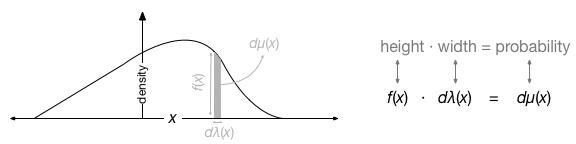
\includegraphics[width=1\textwidth,height=\textheight]{images/radon-nikodym.png}

}

\caption{Change of measures.}

\end{figure}%

확률측도는 volume element의 일반화라고 볼 수 있다.

\begin{itemize}
\item
  \(\mu(x)\): probability measure, interval이나 set of points들을
  인풋으로 받고 area/volume에 해당하는 확률(양수)을 아웃풋으로 주는
  함수다.
\item
  \(\lambda (x)\): reference measure. We often take \(\lambda (x)\) as
  the Lebesgue measure which is essentially just a uniform function over
  the sample space.
\end{itemize}

The reference measure \(\lambda (x)\) is essentially just a meter-stick
that allows us to express the probability measure as a simple function
\(f(x)\). That is, we represent the probability measure \(\mu(x)\) as
\(f(x)\) by comparing the probability measure to some specified
reference measure \(\lambda (x)\). This is essentially the intuition
that is given by the Radon-Nikodym derivative \[
f(x) = \frac{d\mu (x)}{d\lambda (x)}
\] or equivalently \[
\text{height = area / width.}
\] Note that we can also represent the same idea by \[
\mu (A) = \int_{A\in X} f(x) d\lambda (x),
\] where \(\mu(A)\) is the sum of the probability of events in the set
\(A\) which is itself a subset of the entire sample space \(X\). Note
that when \(A=X\) then the integral must equal \(1\) by definition of
probability.

라돈-니코딤 정리는 조건부 확률에 응용된다고 함.

\section{Integration}\label{integration}

\section{리만-스틸체스
적분}\label{uxb9acuxb9cc-uxc2a4uxd2f8uxccb4uxc2a4-uxc801uxbd84}

종종 헷갈리는 표현이 기댓값을 다음과 같이 분포함수를 이용해 표현하는
경우가 있다.

\[
E(X) = \int x dF(x).
\]

우리가 알고 있는 정적분은 \(x\)축을 따라가며 함수값 f(x)가 만드는 면적을
계산한다.

\[
\int_a^b f(x) dx.
\]

위 식을 더 확장하면 \(x\) 대신 임의의 곡선 \(g(x)\)를 적분 변수로 두고
\(f(x)\) 를 단순하게 정적분 할 수도 있다.

\[
\int_{x=a}^b f(x) dg(x).
\]

여기서 \(dg(x)\)는 \(g(x)\)의 미분소(differential)로, \(g(x)\)의
움직임을 결정하는 \(x\)는 단조 증가하거나 감소한다. 위와 같이 리만
적분을 일반화한 정적분을 \textbf{리만-스틸체스 적분(Riemann-Stieltjes
Integral)}이라 한다. 리만 적분의 정의를 이용해 리만-스틸체스의 적분을
표현할 수도 있다.

\[
\int_{x=a}^b f(x) dg(x) = \lim_{N\rightarrow \infty} \sum_{n=0}^{N-1} f(t_n) [g(x_{n+1}) - g(x_n)].
\]

여기서 \(x_n\)은 정적분을 위해 구간 \([a,b]\)를 나눈 점, \(t_n\)은 닫힌
세부공간 \([x_n, x_{n+1} ]\)사이에 있는 임의점이다.

\section{리만 적분과 르베그
적분}\label{uxb9acuxb9cc-uxc801uxbd84uxacfc-uxb974uxbca0uxadf8-uxc801uxbd84}

여기는
\href{https://math.stackexchange.com/questions/2958787/confused-when-changing-from-lebesgue-integral-to-riemann-integral}{Confused
when changing from Lebesgue Integral to Riemann Integral} 에 올라왔던
내용을 살펴보기로 한다. 여기서 질문자는 리만 적분을 어떻게 르베그
적분으로 바꾸는지에 대해 관심이 있다.

다음과 같이 확률공간 \((\Omega, \mathcal{F}, P)\)에서 정의된 음이 아닌
확률변수 \(X\)가 지수분포를 따른다고 하자. \[
P(X<x) = 1-e^{-\lambda x}.
\] 한편, 르베그 적분으로 \(X\)의 기댓값을 쓰면 다음과 같다. \[
E[X] = \int_{\{\omega | X(\omega) \geq 0 \}} X(\omega) dP(\omega).
\] 여기서 질문자는 이것을 리만 적분으로 어떻게 바꾸냐 \[
E[X] = \int_0^\infty x \lambda e^{-\lambda x}dx
\] 를 물어보고 있다.

답변은 이것이 적분의 문제가 아닌 변수변환의 문제라고 한다.

By definition, given \(X: \Omega \rightarrow \mathbb{R}\) a random
variable, \(E[X] = \int_{\Omega} X\). \(X\) defines a measure
\(\tilde{m}\) in \(\mathbb{R}\), called the \textbf{push-forward}, by
\(\tilde{m}(A) = P(X^{-1}(A))\). By definition, this measure is
invariant under \(X\), and hence \[
\int_{\mathbb{R}} f d\tilde{m} = \int_{\Omega} f \circ X dP.
\] The equality follows from the usual arguments (prove for
characteristics, simple functions, then use convergence. Recall that
\(1_A \circ X = 1_{X^{-1}(A)}\)).

Let \(h\) be the density of \(X\). We then have, by definition of
density, that \(\tilde{m}(A) = P(X^{-1}(A)) = \int_A h dm\) for any
\(A \in \mathcal{B}(\mathbb{R})\), where \(m\) is the Lebesgue measure.
By \textbf{change of variables}, we have \[
\int_{\mathbb{R}}f d\tilde{m} = \int_{\mathbb{R}} f\cdot h dm.
\] Combining these equations, \[
\int_{\mathbb{R}} f \cdot h dm =\int_{\Omega} f \circ X dP.
\] Taking \(f=\text{Id}\) yields \[
\int_{\mathbb{R}}xh(x)dx = \int_{\Omega} X dP = E[X].
\] Taking \(f = \text{Id} \cdot \mathbf{1}_{I}\), where \(I\) is some
interval (for example, \((0, +\infty)\) as in your case), we have \[
\int_{I}xh(x)dx = \int_{X^{-1}}XdP,
\] recalling again that
\(\mathbf{1}_A \circ X = \mathbf{1}_{X^{-1}(A)}\). Since \(P(X<0)\) in
your case is \(0\), this last integral is actually equal to the integral
over the whole space, and hence to \(E[X]\), which gives your equality.

\begin{definition}[Integrable Random
Variable]\protect\hypertarget{def-integrablerv}{}\label{def-integrablerv}

Gut (2014) 의 53쪽에 따르면, \(E|X|<\infty\)인 경우 random varible
\(X\)가 integrable 하다고 부른다.

\end{definition}

\begin{example}[]\protect\hypertarget{exm-lebesgueprob}{}\label{exm-lebesgueprob}

Given a probability measure \(P\) and sample space \(\Omega\), it is
true that \[
\int_{\Omega} dP = 1.
\] Because \[
\int_{\Omega} dP = P(\Omega) = 1.
\] More generally \[
\int_A dP = \int_{\Omega} 1_A dP = P(A), \quad{} A \in \mathcal{F}.
\]

\end{example}

\begin{definition}[\(\mathcal{L}^p\)]\protect\hypertarget{def-Lp}{}\label{def-Lp}

다음과 같은 확률공간 \((\Omega, \mathcal{F}, P)\)를 생각하자. \(p>1\)에
대해, 확률변수 \(X\)가 \(E|X|^p < \infty\)이면
\(X\in \mathcal{L}^p\)\index{$L^p$수렴}라고 하며 다음과 같은 놈
\(\|X_p\| = (E|X|^p)^{\frac{1}{p}}\)를 정의할 수 있다.

\end{definition}

\chapter{Probability Inequalities}\label{probability-inequalities}

\section{왜 concentration inequality가
필요한가?}\label{uxc65c-concentration-inequalityuxac00-uxd544uxc694uxd55cuxac00}

\begin{itemize}
\tightlist
\item
  출처:
  \href{https://gclinderman.github.io/blog/probability/2018/01/07/concentration-inequalities.html}{Concentration
  Inequalities}
\end{itemize}

\begin{itemize}
\item
  \href{https://www.math.uci.edu/~rvershyn/papers/HDP-book/HDP-book.html}{High-Dimensional
  Probability} 책에 있는 동전 던지기 예제 생각
\item
  \(i\)번째 동전던지기: 앞면이 나오면 1, 뒷면이 나오면 0인 Bernoulli
  random variable로 간주 가능
\item
  \(N\)번 던졌을 때 나온 앞면의 수: \(S_N = \sum_i X_i\)
\item
  de Moivre-Laplace theorem (Binomial의 CLT) \[
  Z_N \stackrel{D}{\rightarrow}\mathcal{N}(0,1)
  \] 이때 \[
  Z_N  = \frac{S_N - N_p}{\sqrt{Np (1-p)}}
  \]
\end{itemize}

\begin{figure}[H]

{\centering 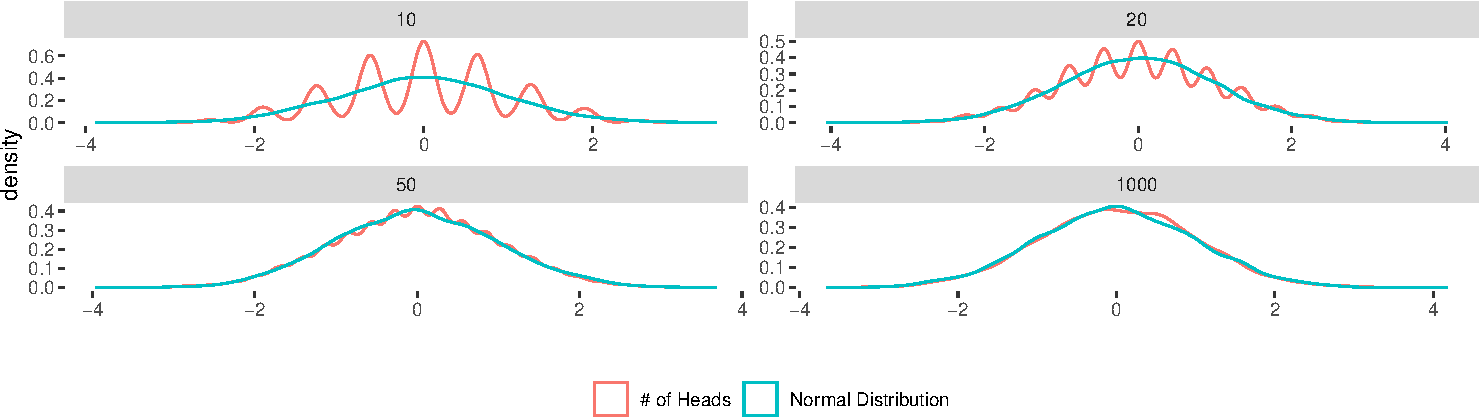
\includegraphics[width=0.7\textwidth,height=\textheight]{ineq_files/figure-pdf/unnamed-chunk-2-1.pdf}

}

\caption{Figure: CLT 묘사.}

\end{figure}%

\textbf{Q}. \(N\)번 시행 시 \(\frac{3}{4}\)이상 앞면이 나올 확률을
구하고 싶다.

\begin{itemize}
\item
  Gaussian density는 exponential decay하는데, \(Z_N\)이 분포수렴하는
  속도는 훨씬 느림
\item
  CLT의 quantitative version인 Berry-Essen CLT를 보면 \[
  |P\{Z_n \geq t\} - P\{Z \geq t\} | \leq \frac{C}{\sqrt{N}}
  \] 이때 \(C\)는 상수이며, convergence의 order가
  \(\frac{1}{\sqrt{N}}\)임을 (아래 그림에 녹색으로 표시) 확인 가능
\end{itemize}

\begin{figure}[H]

{\centering 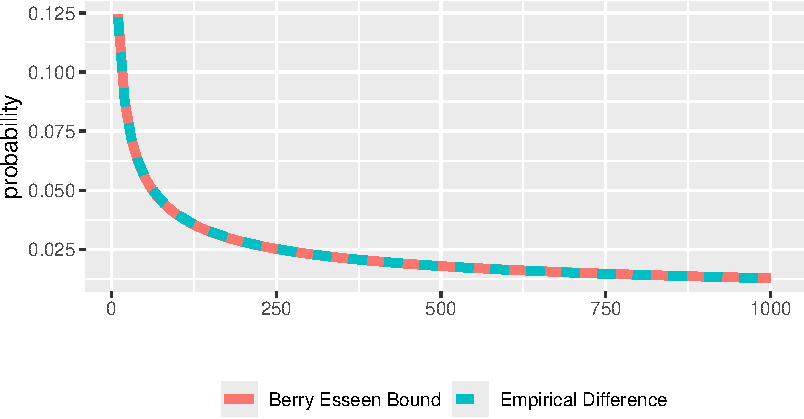
\includegraphics[width=0.7\textwidth,height=\textheight]{ineq_files/figure-pdf/unnamed-chunk-3-1.pdf}

}

\caption{Figure: Berry-Essen bound와 empirical difference.}

\end{figure}%

\section{Markov inequality}\label{markov-inequality}

\begin{theorem}[Markov
inequality]\protect\hypertarget{thm-markovineq}{}\label{thm-markovineq}

음이 아는 확률변수 \(X\)에 대해 \[
P\{ X\geq t\} \leq \frac{E[X]}{t}
\]

\end{theorem}

\begin{tcolorbox}[enhanced jigsaw, opacityback=0, colframe=quarto-callout-tip-color-frame, breakable, left=2mm, arc=.35mm, rightrule=.15mm, titlerule=0mm, coltitle=black, title=\textcolor{quarto-callout-tip-color}{\faLightbulb}\hspace{0.5em}{Proof}, colbacktitle=quarto-callout-tip-color!10!white, toptitle=1mm, bottomtitle=1mm, leftrule=.75mm, toprule=.15mm, colback=white, opacitybacktitle=0.6, bottomrule=.15mm]

확률공간 \((\Omega, \Sigma, P)\)을 생각하자. \[
EX = \int X dP \geq \int_{\{X\geq t\}} X dP \geq t \int_{\{X\geq t \}}dP \geq t\cdot P\{ X\geq t\}
\]

\end{tcolorbox}

\begin{tcolorbox}[enhanced jigsaw, opacityback=0, colframe=quarto-callout-note-color-frame, breakable, left=2mm, arc=.35mm, rightrule=.15mm, titlerule=0mm, coltitle=black, title=\textcolor{quarto-callout-note-color}{\faInfo}\hspace{0.5em}{Remark}, colbacktitle=quarto-callout-note-color!10!white, toptitle=1mm, bottomtitle=1mm, leftrule=.75mm, toprule=.15mm, colback=white, opacitybacktitle=0.6, bottomrule=.15mm]

\begin{itemize}
\item
  마르코프 bound는 매우 약한 (즉 true probabilty로의 수렴이 느린) bound
\item
  그러나 \(X\)에 대한 제약조건이 없음 (기댓값 계산 필요, 음이 아닌
  확률변수)
\end{itemize}

\end{tcolorbox}

\section{Chebyshev inequality}\label{chebyshev-inequality}

\begin{theorem}[Chebyshev
inequality]\protect\hypertarget{thm-chevyshevineq}{}\label{thm-chevyshevineq}

어떤 확률변수 \(X\)에 대해 \[
P\{|X-E(X)|\geq t \}\leq \frac{\text{Var}(X)}{t^2}
\]

\end{theorem}

\begin{tcolorbox}[enhanced jigsaw, opacityback=0, colframe=quarto-callout-tip-color-frame, breakable, left=2mm, arc=.35mm, rightrule=.15mm, titlerule=0mm, coltitle=black, title=\textcolor{quarto-callout-tip-color}{\faLightbulb}\hspace{0.5em}{Proof}, colbacktitle=quarto-callout-tip-color!10!white, toptitle=1mm, bottomtitle=1mm, leftrule=.75mm, toprule=.15mm, colback=white, opacitybacktitle=0.6, bottomrule=.15mm]

\(|X-E(X)|\geq t\)를 제곱한 후 마르코프 부등식을 적용 \[
P\{ |X-E(X)|^2 \geq t^2\} \leq \frac{E[(X-E(X))]^2}{t^2} = \frac{\text{Var}(X)}{t^2}
\]

\end{tcolorbox}

\begin{tcolorbox}[enhanced jigsaw, opacityback=0, colframe=quarto-callout-note-color-frame, breakable, left=2mm, arc=.35mm, rightrule=.15mm, titlerule=0mm, coltitle=black, title=\textcolor{quarto-callout-note-color}{\faInfo}\hspace{0.5em}{Remark}, colbacktitle=quarto-callout-note-color!10!white, toptitle=1mm, bottomtitle=1mm, leftrule=.75mm, toprule=.15mm, colback=white, opacitybacktitle=0.6, bottomrule=.15mm]

\begin{itemize}
\tightlist
\item
  체비세프 부등식을 쓰려면 분산이 정의되어야 함
\end{itemize}

\end{tcolorbox}

\section{Hoeffding's Inequality}\label{hoeffdings-inequality}

\begin{itemize}
\item
  (드디어) \(\sum_i X_i\)에 대한 exponential bound를 줌
\item
  그러나 독립 가정이 필요
\item
  단순한 케이스로 먼저 \(X_1, \ldots, X_N\)이 symmetric Bernoulli라고
  하자. 이는 즉 반반의 확률로 1 또는 -1을 갖는 확률변수
\end{itemize}

\begin{theorem}[Symmetric Bernoulli에서의 Hoeffding's
inequality]\protect\hypertarget{thm-hoeffdingbernoulli}{}\label{thm-hoeffdingbernoulli}

\(X_1, \ldots, X_N\)이 symmetric Bernoulli 확률변수라고 하자. 어떤
\(t\geq 0\)에 대해 \(a \in \mathbb{R}^n\)이 존재해 \[
P\{ \sum_{i=1}^N a_i X_i \geq t \} \leq \exp \Big( - \frac{t^2}{2\|a\|^2} \Big)
\]

\end{theorem}

\begin{tcolorbox}[enhanced jigsaw, opacityback=0, colframe=quarto-callout-tip-color-frame, breakable, left=2mm, arc=.35mm, rightrule=.15mm, titlerule=0mm, coltitle=black, title=\textcolor{quarto-callout-tip-color}{\faLightbulb}\hspace{0.5em}{Proof}, colbacktitle=quarto-callout-tip-color!10!white, toptitle=1mm, bottomtitle=1mm, leftrule=.75mm, toprule=.15mm, colback=white, opacitybacktitle=0.6, bottomrule=.15mm]

마르코프 부등식을 적용하면 다음과 같다. \[
P\{ \sum_{i=1}^N a_i X_i \geq t \} = P \{ \exp (\lambda \sum_{i=1}^N a_i X_i) \geq e^{\lambda t} \} \leq e^{-\lambda t}E\{ \exp (\lambda \sum_{i=1}^N a_i X_i) \}
\] 독립성에 의해 다음과 같다. \[
E\{ \exp (\lambda \sum_{i=1}^N a_i X_i) \} = E \{ \prod_{i=1}^N \exp (\lambda a_i X_i)  \} = \prod_{i=1}^N E\{ \exp (\lambda a_i X_i)\}
\] \(X_i\)를 \(1/2\)의 확률로 -1과 1을 갖는 확률변수라고 제한했으므로,
위의 기댓값을 쉽게 구할 수 있다. \[
E\{ \exp (\lambda a_i X_i)\} = \frac{e^{\lambda a_i }+ e^{-\lambda a_i}}{2}\leq e^{\lambda^2 a_i^2 / 2}
\] 지수함수의 테일러 급수 전개를 이용하면 \[
e^{x}=\sum_{k=0}^{\infty}\frac{x^k}{k!},\quad{} \frac{e^{x}+e^{-x}}{2} =\sum_{k=0}^{\infty}\frac{x^{2k}}{(2k)!}, \quad{} e^{x^2/2}=\sum_{k=0}^{\infty}\frac{x^{2k}}{2^k k!},\quad{} \Longrightarrow\quad{} \frac{e^{x}+e^{-x}}{2} \leq e^{x^2/2}.
\] \(\|a\|^2=1\)이라 두고 위의 결과를 대입해보자. \[
P\{ \sum_{i=1}^N a_i X_i \geq t \} \leq e^{-\lambda t}(\prod_{i=1}^N e^{\lambda^2 a_i^2/2})\leq e^{-\lambda t}(e^{\lambda^2 \sum_{i=1}^N a_i^2/2}) = e^{-\lambda t}(e^{\lambda^2/2}) = e^{\lambda^2/2 - \lambda t}.
\] 위의 부등식은 모든 \(\lambda\)에 대해 성립하고, \(\lambda=t\)일 때
최소화된다. 따라서 \[
P\{ \sum_{i=1}^N a_i X_i \geq t \} \leq e^{-t^2/2}.
\] 따라서, homogeneity에 의해 \(\|a\|=1\)을 가정하면 다음과 같다. \[
P \{ \sum_{i=1}^N \frac{a_i}{\| a\|}X_i \geq \frac{t}{\|a\|} \} \leq e^{-\frac{t^2}{2\|a\|^2}}.
\]

\end{tcolorbox}

\(X_i\)가 1 또는 0을 갖는 베르누이 확률변수라고 할 때,
\(Y_i = 2(X_i - \frac{1}{2})\)로 놓으면 \(Y_i\)는 symmetric Bernoulli
확률변수임 \[
P\{ \sum_i X_i > t\} = P \{ \sum_i (\frac{Y_i}{2}+ \frac{1}{2}) > t \} = P\{\sum_i Y_i > 2t - N \} \leq \exp (-\frac{(2t-N)^2}{2N})
\] 여기서 \(a=\begin{bmatrix} 1,1,\ldots, 1 \end{bmatrix}\)로 두면
\(\|a\|_2^2=N\)이 된다. 따라서 \[
P\{\sum_i X_i > \frac{3N}{4} \}\leq \exp (- \frac{(\frac{3N}{2}-N)^2}{2N}) = \exp (-\frac{N}{8})
\]

\begin{figure}[H]

{\centering 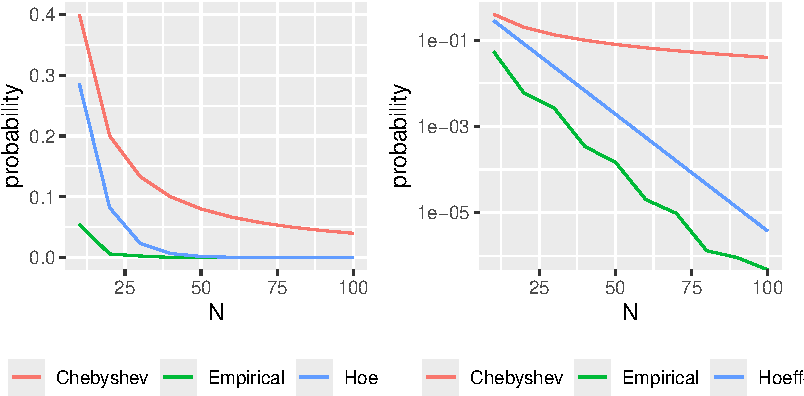
\includegraphics[width=0.7\textwidth,height=\textheight]{ineq_files/figure-pdf/unnamed-chunk-4-1.pdf}

}

\caption{Figure: Chebyshev와 Hoeffding bound의 비교.}

\end{figure}%

\begin{theorem}[Hoeffding's
inequality]\protect\hypertarget{thm-hoeffdingineq}{}\label{thm-hoeffdingineq}

\(X_1, \ldots, X_N\)이 독립인 확률변수이고, \(X_i \in [m_i, M_i]\)
almost surely라고 하자. 그러면 어떤 \(t>0\)에 대해 \[
P \{\sum_{i=1}^N (X_i - E(X_i))\geq t \} \leq \exp (- \frac{2t^2}{\sum_{i=1}^N (M_i - m_i)^2})
\]

\end{theorem}

\begin{tcolorbox}[enhanced jigsaw, opacityback=0, colframe=quarto-callout-tip-color-frame, breakable, left=2mm, arc=.35mm, rightrule=.15mm, titlerule=0mm, coltitle=black, title=\textcolor{quarto-callout-tip-color}{\faLightbulb}\hspace{0.5em}{Proof}, colbacktitle=quarto-callout-tip-color!10!white, toptitle=1mm, bottomtitle=1mm, leftrule=.75mm, toprule=.15mm, colback=white, opacitybacktitle=0.6, bottomrule=.15mm]

앞에서처럼 \(\lambda\)를 곱하고 제곱근을 취한 다음 마르코프 부등식을
이용한다 \[
\begin{align*}
P\{\sum (X_i - E(X_i)) \geq t \} &= P \{\exp (\lambda \sum (X_i - E(X_i)))\geq e^{\lambda t} \}\\
&\leq E \{\exp (\lambda \sum (X_i - E(X_i)))\} e^{-\lambda t}\\
&= \prod_i E\{\exp (\lambda (X_i - E(X_i))) \}e^{-\lambda t}.
\end{align*}
\] 그러면 기댓값의 bound만 찾아주면 된다. 여기서는 \(X_i\)와 독립인
copy인 \(X_i'\)를 생각하는 \textbf{symmetrization} 기법을 이용한다. \[
\begin{align*}
E\{\exp (\lambda \sum (X_i - E(X_i)) ) \} &= E\{\exp (\lambda \sum (X_i - E(X_i')) ) \} \\
&= E_{X_i} \{ \exp (E_{X_i'} \lambda \sum (X_i - X_i')) \}\\
&\leq E_{X_i} E_{X_i'} \{ \exp (\lambda \sum (X_i - X_i')) \}\\
&= E\{ \exp (\lambda \sum (X_i - X_i')) \}.
\end{align*}
\] 여기서 exponential이 convex이므로 Jensen의 부등식을 적용하였다.
여기서 \(X_i - X_i'\)는 0 근처에서 symmetric이고 이것의 분포는
\(S(X_i - X_i')\)와 같다. 이때 \(S\)는 -1, 1을 동일한 확률로 갖는
\textbf{Rademacher variable}이다. \[
\begin{align*}
E\{\exp (\lambda \sum (X_i - E(X_i)) ) \} &\leq E_{X_i,X_i'} \{ E_S \exp (\lambda \sum S(X_i - X_i')) \}\\
&\leq E_{X_i,X_i'} \{ \exp (\lambda^2 (X_i - X_i')^2/2) \}\\
&\leq \exp (\lambda^2 (M_i - m_i)^2/2).
\end{align*}
\] 이때 첫 번째 부등식은 exponential의 테일러 전개를, 두 번째 부등식은
\(X_i\)의 boundedness를 이용하였다. \[
\begin{align*}
P\{\sum (X_i - E(X_i)) \geq t \} &=  \prod_i E\{\exp (\lambda (X_i - E(X_i))) \}e^{-\lambda t}\\
&= \prod_i \exp (\lambda^2 (M_i - m_i)^2/2)e^{-\lambda t}\\
&= \exp (\lambda^2 \sum_i (M_i - m_i)^2/2 -\lambda t)\\
&\leq \exp (\frac{2t^2}{\sum_i (M_i -m_i)^2}).
\end{align*}
\] 여기서 마지막 부등식은 exponent를 최소화하는 \(\lambda\)를 잡았다.

\end{tcolorbox}

\section{Chernoff Bounds}\label{chernoff-bounds}

\begin{itemize}
\item
  베르누이 확률변수에 대한 Hoeffding bound는 \(p=0.5\)일 때에는 잘
  작동하지만, 작거나 큰 \(p\)에 대해서는 잘 작동하지 않음
\item
  \(X_i \sim \text{Bernoulli}(p)\)라고 하고
  \(S_N = \sum_{i=1}^N X_i\)라고 두자. 그리고 Hoeffding의 부등식을
  이용하여 \(S_N > 10pN\)의 bound를 구해보자. \[
  P \{ \sum_i X_i > 10pN \} = P\{ \sum_i X_i - pN > 9pN \}\leq \exp (-\frac{2(9pN)^2}{N}) = \exp (-182p^2 N).
  \] 식을 보면 Binomial random variable이 평균보다 9배 클 확률의 bound를
  계산함
\end{itemize}

\begin{theorem}[Chernoff
inequality]\protect\hypertarget{thm-chernoffineq}{}\label{thm-chernoffineq}

\(X_1, \ldots, X_N\)이 모수 \(p_i\)를 갖는 독립인 베르누이 확률변수라
하자. \(S_N = \sum_i X_i\)이고 \(\mu = E(S_N)\)이라고 하자. 그러면
\(t>\mu\)에 대해 \[
P \{ S_N \geq t \} \leq \exp (-\mu) \Big( \frac{e\mu}{t} \Big)^t.
\]

\end{theorem}

\begin{tcolorbox}[enhanced jigsaw, opacityback=0, colframe=quarto-callout-tip-color-frame, breakable, left=2mm, arc=.35mm, rightrule=.15mm, titlerule=0mm, coltitle=black, title=\textcolor{quarto-callout-tip-color}{\faLightbulb}\hspace{0.5em}{Proof}, colbacktitle=quarto-callout-tip-color!10!white, toptitle=1mm, bottomtitle=1mm, leftrule=.75mm, toprule=.15mm, colback=white, opacitybacktitle=0.6, bottomrule=.15mm]

다시 \(\lambda\)를 곱하고 마르코프 부등식을 적용하자. \[
P\{ S_N \geq t \} \leq E\{ \exp (\lambda \sum_{i} X_i) \}e^{-\lambda t} = \prod_i E\{ \exp (\lambda X_i) \}e^{-\lambda t}.
\] \(1+x \leq e^{x}\)라는 부등식을 이용하면 다음과 같다. \[
P\{ S_N \geq t \} \leq  e^{\lambda}p_i + (1-p_i) = 1 + (e^{\lambda} - 1)p_i \leq \exp (p_i (e^\lambda - 1)).
\] 이것을 정리하면 다음과 같다. \[
\begin{align*}
P\{ S_N \geq t \} &\leq \prod_i \exp (p_i (e^\lambda -1))e^{-\lambda t}\\
&\leq \exp \Big( (e^\lambda - 1)\sum_i p_i \Big) e^{-\lambda t}\\
&\leq \exp ((e^{\lambda}-1)\mu) e^{-\lambda t}.
\end{align*}
\] 여기서 \(\lambda\)를 고를 수 있는데, \(\lambda = \log (t/mu)\)로
잡으면 다음과 같다. \[
\begin{align*}
P\{ S_N \geq t \} &\leq \exp \Big( (\frac{t}{\mu}-1)\mu \Big) \Big( \frac{\mu}{t} \Big)^t\\
&= \exp (t-\mu) \Big( \frac{\mu}{t} \Big)^t\\
&=\exp (-\mu) \Big( \frac{e\mu}{t} \Big)^t.
\end{align*}
\]

\end{tcolorbox}

\begin{itemize}
\tightlist
\item
  다시 앞 예제에 Chernoff 부등식을 적용하면 \[
  P \{\sum_i X_i > 10pN \} \leq \exp (-p N) \Big( \frac{epN}{10pN}\Big)^{10pN} = \exp (-p N) \Big( \frac{e}{10}\Big)^{10pN}.
  \]
\end{itemize}

\begin{figure}[H]

{\centering 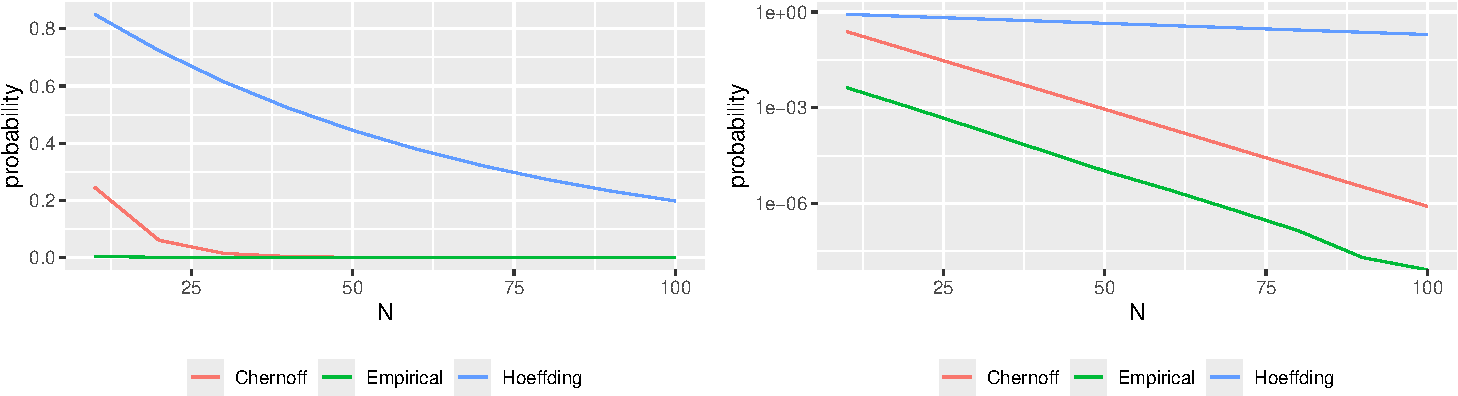
\includegraphics[width=0.7\textwidth,height=\textheight]{ineq_files/figure-pdf/unnamed-chunk-5-1.pdf}

}

\caption{Figure: Hoeffding과 Chernoff bound의 비교.}

\end{figure}%

\section{Gaussian tails and MGF}\label{gaussian-tails-and-mgf}

\begin{itemize}
\item
  출처:
  \href{https://ocw.mit.edu/courses/18-s997-high-dimensional-statistics-spring-2015/a69e2f53bb2eeb9464520f3027fc61e6_MIT18_S997S15_Chapter1.pdf}{High-Dimensional
  Statistics Lecture Notes}
\item
  \(X\)가 Gaussian일 때 pdf \[
  p(x) = \frac{1}{\sqrt{2\pi \sigma^2}} \exp \Big( - \frac{(x-\mu)^2}{2\sigma^2} \Big), \quad{} x \in \mathbb{R}
  \]
\item
  Bounded support: \(P(|X-\mu|\leq 3\sigma)\) 등의 확률 구할 때 사용
\end{itemize}

\begin{proposition}[Gaussian의 tail
probability]\protect\hypertarget{prp-gaussiantail}{}\label{prp-gaussiantail}

\(X\sim \mathcal{N}(\mu, \sigma^2)\)일 때 \(t>0\)에 대해 \[
P(|X-\mu | >t) \leq \sqrt{\frac{2}{\pi}}\frac{e^{-\frac{t^2}{2\sigma^2}}}{t}.
\]

\end{proposition}

\section{Sub-Gaussian}\label{sub-gaussian}

\begin{itemize}
\item
  출처:
  \href{https://gclinderman.github.io/blog/probability/2018/01/07/concentration-inequalities.html}{Concentration
  Inequalities}
\item
  앞서 Chernoff appraoch로 얻어지는 tail bound의 form은 MGF의 growth
  rate에 depend됨을 암
\item
  따라서 tail bound study에서는 확률변수들을 MGF에 따라 분류하는 것이
  자연스러운 생각
\end{itemize}

\begin{definition}[Sub-Gaussian]\protect\hypertarget{def-subgaussian}{}\label{def-subgaussian}

어떤 확률변수 \(X\in \mathbb{R}\)이 \(E(X)=0\)이고 이것의 MGF가 \[
E[\exp (sX)] \leq \exp \Big( \frac{\sigma^2 s^2}{2} \Big), \forall s \in \mathbb{R}
\] 일 때 \(X \sim \text{subG}(\sigma^2)\)이라고 한다.

\end{definition}

\begin{tcolorbox}[enhanced jigsaw, opacityback=0, colframe=quarto-callout-note-color-frame, breakable, left=2mm, arc=.35mm, rightrule=.15mm, titlerule=0mm, coltitle=black, title=\textcolor{quarto-callout-note-color}{\faInfo}\hspace{0.5em}{Remark}, colbacktitle=quarto-callout-note-color!10!white, toptitle=1mm, bottomtitle=1mm, leftrule=.75mm, toprule=.15mm, colback=white, opacitybacktitle=0.6, bottomrule=.15mm]

\begin{itemize}
\tightlist
\item
  Sub-Gaussian random variable은 클래스가 큼
\end{itemize}

\end{tcolorbox}

\section{Sub-Exponential}\label{sub-exponential}

\begin{itemize}
\item
  \(X\sim \text{Lap}(1)\)과 같이 \[
  P(|X|>t)=e^{-t},\quad{} t\geq 0
  \] Gaussian보다 꼬리가 두꺼운 경우는 어떻할 것인가?
\item
  Laplace의 MGF: \[
  E[e^{sX}] = \frac{1}{1-s^2},\quad{} \text{if } |s|<1.
  \]
\end{itemize}

\begin{definition}[Sub-Exponential]\protect\hypertarget{def-subexponential}{}\label{def-subexponential}

어떤 확률변수 \(X\in \mathbb{R}\)이 \(E(X)=0\)이고 이것의 MGF가 \[
E[e^{sX}] \leq e^{s^2 \lambda^2 / 2}, \quad{} \forall |s| \leq \frac{1}{\lambda}
\] 일 때 \(X \sim \text{subE}(\lambda)\)라고 한다.

\end{definition}

\section{Bernstein's inequality}\label{bernsteins-inequality}

\begin{theorem}[Berstein's
inequality]\protect\hypertarget{thm-bersteinineq}{}\label{thm-bersteinineq}

어떤 확률변수 \(X_1, \ldots, X_n\)이 독립이고 \(E(X_i) = 0\)이며
\(X_i \sim \text{subE}(\lambda)\)인 확률변수라고 하자. 그러면 \(t>0\)에
대해 \[
P(\overline{X} >t) \vee P(\overline{X} < -t) \leq \exp \Big[ - \frac{n}{2}\Big(\frac{t^2}{\lambda^2}\wedge \frac{t}{\lambda} \Big) \Big] .
\]

\end{theorem}

\chapter{Convergence}\label{convergence}

이 장에서는 확률변수의 수렴에 대해 알아본다. \(X_1, X_2, \ldots\)가
확률변수라고 하자.

\begin{itemize}
\item
  그러면 만약 이들 \(n\)항까지의 합 \(S_n\)은 \(n\rightarrow\infty\)일
  때 어떻게 될 것인가?
\item
  \(\max \{X_1,\ldots, X_n\}\)은 \(n\rightarrow\infty\)일 때 어떻게 될
  것인가?
\item
  수열의 극한은 어떠할 것인가?
\item
  수열의 함수는 어디로 수렴할 것인가? 이는 수학에서 적분의 수렴에
  대응된다고 한다. (Gut 2014)
\item
  적분의 극한은 극한의 적분과 같을 것인가?
\end{itemize}

\section{Definitions}\label{definitions}

다음의 정의들은 확률론에서 많이 등장하는 정의들이다.
\(X_1,X_2,\ldots\)를 확률변수열이라 하자.

\section{Almost Sure Convergence}\label{almost-sure-convergence}

\begin{definition}[Sure convergence (틀림없는
수렴)]\protect\hypertarget{def-sconv}{}\label{def-sconv}

확률변수열 \(X_n\)이 표본공간 안에 어떤 점 \(\omega\)를 잡아도 \[
\lim_{n\rightarrow\infty} X_n (\omega) = X(\omega)
\] 을 만족하면 \(X_n\) \textbf{converges surely (a.s.)} to the random
variable \(X\) as \(n\rightarrow \infty\)라 하고,
\(X_n \stackrel{\text{s}}{\rightarrow}X\) as \(n\rightarrow \infty\)라
쓴다.

\end{definition}

\begin{definition}[Almost sure convergence (거의 틀림없는
수렴)]\protect\hypertarget{def-asconv}{}\label{def-asconv}

확률변수열 \(X_n\)은 \[
P\{ \omega: X_n (\omega)\rightarrow X(\omega) \text{ as } n\rightarrow \infty\})=1
\] 을 만족하면 \(X_n\) \textbf{converges almost surely (a.s.)} to the
random variable \(X\) as \(n\rightarrow \infty\)라 하고,
\(X_n \stackrel{\text{a.s.}}{\rightarrow}X\) as
\(n\rightarrow \infty\)라 쓴다.

\end{definition}

\begin{tcolorbox}[enhanced jigsaw, opacityback=0, colframe=quarto-callout-note-color-frame, breakable, left=2mm, arc=.35mm, rightrule=.15mm, titlerule=0mm, coltitle=black, title=\textcolor{quarto-callout-note-color}{\faInfo}\hspace{0.5em}{Remark}, colbacktitle=quarto-callout-note-color!10!white, toptitle=1mm, bottomtitle=1mm, leftrule=.75mm, toprule=.15mm, colback=white, opacitybacktitle=0.6, bottomrule=.15mm]

\begin{itemize}
\item
  거의 틀림없이 수렴하는 확률변수 \(\{ X_n (\omega)\}\)에서는
  \(P(\tilde{\Omega})=1\)이고 \(\tilde{\Omega} \subseteq \Omega\)일 때
  \(\omega \in \tilde{\Omega}\)를 어떻게 고르더라도
  \(\lim_{n\rightarrow \infty} X_n (\omega) = X(\omega)\)임
\item
  다만, \(\omega \notin \tilde{\Omega}\)인 수열 \(\{ X_n (\omega)\}\)는
  수렴하지 않을 수는 있지만,
  \(P\{ \omega: \omega \notin \tilde{\Omega}, \omega \in \Omega\} = 0\)임
\item
  \(X_n \stackrel{\text{a.s.}}{\rightarrow}0\)은 \(0\)보다 큰 수
  \(\varepsilon\)을 어떻게 잡더라도
  \(P\{ |X_n| \geq \varepsilon\} =0\)이라는 것과 필요충분조건임
\end{itemize}

\end{tcolorbox}

\begin{example}[거의 틀림없는 수렴
예제]\protect\hypertarget{exm-asconv01}{}\label{exm-asconv01}

~

\begin{itemize}
\tightlist
\item
  구간 \([0,1]\)에서 아무렇게나 한 점을 골라서 \(\omega\)라 하고,
  \(\omega\)가 \([0,1]\)의 어느 부분 구간에 들어갈 확률은 그 부분 구간의
  길이와 같다고 가정
\end{itemize}

\begin{longtable}[]{@{}
  >{\centering\arraybackslash}p{(\columnwidth - 8\tabcolsep) * \real{0.2000}}
  >{\centering\arraybackslash}p{(\columnwidth - 8\tabcolsep) * \real{0.2000}}
  >{\centering\arraybackslash}p{(\columnwidth - 8\tabcolsep) * \real{0.2000}}
  >{\centering\arraybackslash}p{(\columnwidth - 8\tabcolsep) * \real{0.2000}}
  >{\centering\arraybackslash}p{(\columnwidth - 8\tabcolsep) * \real{0.2000}}@{}}
\toprule\noalign{}
\begin{minipage}[b]{\linewidth}\centering
\(A_n(\omega)\)
\end{minipage} & \begin{minipage}[b]{\linewidth}\centering
\(B_n(\omega)\)
\end{minipage} & \begin{minipage}[b]{\linewidth}\centering
\(C_n(\omega)\)
\end{minipage} & \begin{minipage}[b]{\linewidth}\centering
\(D_n(\omega)\)
\end{minipage} & \begin{minipage}[b]{\linewidth}\centering
\(H_n(\omega)\)
\end{minipage} \\
\midrule\noalign{}
\endhead
\bottomrule\noalign{}
\endlastfoot
\(\frac{\omega}{n}\) & \(\omega (1-\frac{1}{n})\) & \(\omega e^n\) &
\(\cos 2\pi n \omega\) & \(\exp \{ -n (n\omega -1) \}\) \\
\end{longtable}

\begin{itemize}
\item
  \(A_n(\omega)\)는 \(\omega\)가 어떤 값이더라도 늘 0에 수렴하므로
  틀림없이 0에 수렴
\item
  \(B_n(\omega)\)는 \(\omega\)가 어떤 값이더라도 \(\omega\)에 수렴하므로
  틀림없이 \(\omega\)에 수렴하며, 그 극한 분포는 \(U[0,1]\)
\item
  \(C_n (\omega)\)는 \(\omega =0\)이면 0에 수렴하고,
  \(\omega \in (0,1]\)이면 발산, 즉 \(C_n (\omega)\)는 수렴하지 않음
\item
  \(D_n (\omega)\)는 \(\omega \in \{0,1\}\)이면 1에 수렴하고,
  \(\omega \in (0,1)\)이면 -1과 1 사이에서 진동, 즉 \(D_n (\omega)\)는
  수렴하지 않음
\item
  \(\omega=0\)이면 \(H_n (0) = e^n \rightarrow \infty\)이고
  \(\omega \in (0,1]\)이면 \(H_n  (\omega) \rightarrow 0\)이므로
  \(H_n (\omega)\)는 틀림없이 수렴하지는 않지만,
  \(P\{\omega >0\}=1\)이므로 \(H_n (\omega)\)는 거의 틀림 없이 0으로
  수렴
\end{itemize}

\end{example}

\begin{example}[보렐-칸텔리 정리와 거의 어디서나
수렴]\protect\hypertarget{exm-asconv02}{}\label{exm-asconv02}

~

\begin{itemize}
\item
  (\(\Longrightarrow\)) 확률변수 열 \(\{X_n\}_{n=1}^{\infty}\)는
  \(\varepsilon>0\)일 때 \[
  \sum_{n=1}^\infty P\{ |X_n | > \varepsilon\} < \infty
  \] 이면 보렐-칸텔리 정리를 써서 \(n\rightarrow \infty\)일 때
  \(X_n \stackrel{\text{a.s.}}{\rightarrow} 0\)이라는 것을 알 수 있음
\item
  (\(\Longleftarrow\)) \(\omega\)의 분포가 \([0,1]\)에서 고르고 \[
  X_n (\omega)=
  \begin{cases}
  0, & 0 \leq \omega \leq 1-\frac{1}{n},\\
  1, & 1- \frac{1}{n}< \omega \leq 1
  \end{cases}
  \] 인 확률변수 열 \(\{X_n\}_{n=1}^{\infty}\)는
  \(n\rightarrow \infty\)일 때,
  \(X_n \stackrel{\text{a.s.}}{\rightarrow}0\)이다. 그러나
  \(\varepsilon_n \downarrow 0\)인 \(\varepsilon_n\)을 어떻게 잡더라도
  \(n\)이 충분히 크면
  \(P\{ |X_n| > \varepsilon_n \} = P\{ X_n = 1\}= \frac{1}{n}\)이므로
  \(\sum_{n=1}^{\infty}P\{ |X_n| > \varepsilon_n\}\rightarrow \infty\)이다.
  그러므로 앞서 조건은 거의 틀림없이 수렴하는 충분조건이나 필요조건은
  아니다.
\end{itemize}

\end{example}

\begin{theorem}[Almost sure convergence와
동치조건]\protect\hypertarget{thm-asconv}{}\label{thm-asconv}

확률변수 열 \(\{X_n\}_{n=1}^{\infty}\)가
\(X_n \stackrel{\text{a.s}}{\rightarrow}X\)이면 0보다 큰 수
\(\varepsilon\)을 어떻게 고르더라도 \[
\lim_{n\rightarrow\infty} P \{ \sup_{m\geq n} |X_m - X| > \varepsilon \} = 0
\] 이고, 그 역도 성립한다.

\end{theorem}

\begin{tcolorbox}[enhanced jigsaw, opacityback=0, colframe=quarto-callout-note-color-frame, breakable, left=2mm, arc=.35mm, rightrule=.15mm, titlerule=0mm, coltitle=black, title=\textcolor{quarto-callout-note-color}{\faInfo}\hspace{0.5em}{Remark}, colbacktitle=quarto-callout-note-color!10!white, toptitle=1mm, bottomtitle=1mm, leftrule=.75mm, toprule=.15mm, colback=white, opacitybacktitle=0.6, bottomrule=.15mm]

\begin{itemize}
\tightlist
\item
  확률변수 열이 거의 틀림없이 수렴하는지를 보이려면, \(\omega\)의 분포와
  \(\omega\)와 확률변수 사이의 관계를 알든지, 아니면 수렴을 손쉽게 보일
  수 있을 만큼 확률변수가 간단해야 함
\end{itemize}

\end{tcolorbox}

\section{Convergence in Mean}\label{convergence-in-mean}

\textbf{Q}. 거의 틀림없는 수렴보다 조금 더 느슨한 수렴은 없을까?

\begin{definition}[Converge in
\(r\)-mean]\protect\hypertarget{def-rmeanconv}{}\label{def-rmeanconv}

확률변수열 \(X_n\)가 \[
E|X_n - X|^r \rightarrow 0 \quad{} \text{as} \quad{} n\rightarrow \infty.
\] 을 만족하면 \(X_n\) \textbf{converges in} \(r-\)mean to the random
variable \(X\) as \(n\rightarrow \infty\)라 하고,
\(X_n \stackrel{\text{r}}{\rightarrow}X\) as \(n\rightarrow \infty\)
또는 \(X_n \stackrel{L^\text{r}}{\rightarrow}X\) as
\(n\rightarrow \infty\)라 쓴다.

\end{definition}

\begin{tcolorbox}[enhanced jigsaw, opacityback=0, colframe=quarto-callout-note-color-frame, breakable, left=2mm, arc=.35mm, rightrule=.15mm, titlerule=0mm, coltitle=black, title=\textcolor{quarto-callout-note-color}{\faInfo}\hspace{0.5em}{Remark}, colbacktitle=quarto-callout-note-color!10!white, toptitle=1mm, bottomtitle=1mm, leftrule=.75mm, toprule=.15mm, colback=white, opacitybacktitle=0.6, bottomrule=.15mm]

\begin{itemize}
\item
  특별히 \(r=2\)일 때를 제곱 평균 수렴이라 부르며, 해석이 쉽고 공학적인
  응용에서도 많이 쓰임
\item
  제곱 평균 수렴은 어떤 시점 \(n\)에서 \(E\{ (X_n-X)^2\}\)이 작다는
  관점에서 대부분의 수열 \(X_n\)이 \(X\)에 가깝기만 바라는 것임
\item
  이런 수렴은 시간에 중점을 두는 것인데, 거의 틀림없는 수렴과는 달리
  수열 모두의 수렴을 생각하는 것이 아니고, 수렴하는지 아닌지 보이기도 더
  쉬움
\end{itemize}

\end{tcolorbox}

\begin{itemize}
\tightlist
\item
  코쉬 기준: 극한 확률변수 \(X\)를 모를 때에서 확률변수 열이 제곱 평균
  수렴하는지 알아볼 수 있음
\end{itemize}

\begin{theorem}[Cauchy
condition]\protect\hypertarget{thm-cauchycond}{}\label{thm-cauchycond}

확률변수 열 \(\{X_n\}\)이 제곱 평균 수렴할 필요충분조건은 \[
\lim_{n,m\rightarrow\infty} E \{ (X_n - X_m)^2 \} = 0
\] 이다.

\end{theorem}

\begin{example}[]\protect\hypertarget{exm-rmeanconv01}{}\label{exm-rmeanconv01}

~

\begin{itemize}
\item
  Example~\ref{exm-asconv02} 의
  \(B_n(\omega) = (1-\frac{1}{n})\omega\)는 Theorem~\ref{thm-cauchycond}
  를 이용해보면 \[
  \begin{align*}
  \lim_{n,m\rightarrow\infty}E\{(B_n - B_m)^2 \}&= \lim_{n,m\rightarrow\infty}E\{(\frac{1}{n}-\frac{1}{m} )^2 \omega^2 \}\\ &= E\{\omega^2\}\lim_{n,m\rightarrow\infty} (\frac{1}{n}-\frac{1}{m})^2 =0
  \end{align*}
  \] 이므로 코쉬 기준을 만족함을 알 수 있고, 따라서 제곱 평균 수렴할
  것임을 알 수 있음
\item
  또한 다음을 알고 있으므로 \[
  \begin{align*}
  \lim_{n\rightarrow\infty} E[\{ B_n(\omega) - \omega\}^2] &= \lim_{n\rightarrow\infty}E\{ (\frac{\omega}{n})^2 \} \\
  &= \lim_{n\rightarrow\infty}\frac{1}{3n^2}=0
  \end{align*}
  \] \(B_n(\omega)\)는 \(\omega\)에 제곱 평균 수렴
\end{itemize}

\end{example}

\begin{tcolorbox}[enhanced jigsaw, opacityback=0, colframe=quarto-callout-note-color-frame, breakable, left=2mm, arc=.35mm, rightrule=.15mm, titlerule=0mm, coltitle=black, title=\textcolor{quarto-callout-note-color}{\faInfo}\hspace{0.5em}{Remark}, colbacktitle=quarto-callout-note-color!10!white, toptitle=1mm, bottomtitle=1mm, leftrule=.75mm, toprule=.15mm, colback=white, opacitybacktitle=0.6, bottomrule=.15mm]

\begin{itemize}
\tightlist
\item
  제곱 평균 수렴은 \(n\)이 커질 때 점점 더 많은 수열들이 \(X\)에 가까이
  간다는 것을 의미하나, 거의 틀림없는 수렴과 달리 한 번 \(X\)에 가까이
  간 수열이 그 뒤로도 늘 \(X\) 가까이에 머물러 있는 것은 아님
\end{itemize}

\end{tcolorbox}

\begin{example}[]\protect\hypertarget{exm-rmeanconv01}{}\label{exm-rmeanconv01}

~

\begin{itemize}
\tightlist
\item
  Example~\ref{exm-asconv02} 의
  \(H_n(\omega)=\exp \{-n (n\omega - 1) \}\)은 거의 틀림없이 0으로
  수렴하나 \[
  \begin{align*}
  \lim_{n\rightarrow\infty}E[\{ H_n (\omega) - 0 \}^2] &= \lim_{n\rightarrow\infty} e^{2n} \int_{0}^1 \exp (-2n^2 \omega) d\omega\\ &= \lim_{n\rightarrow\infty}\frac{e^{2n}}{2n^2}\{ 1-\exp(-2n^2)\}\rightarrow\infty
  \end{align*}
  \] 이므로 \(\{H_n(\omega)\}\)은 0으로 제곱 평균 수렴하지는 않음
\end{itemize}

\end{example}

\section{Convergence in Probability}\label{convergence-in-probability}

\begin{definition}[Converge in
Probability]\protect\hypertarget{def-pconv}{}\label{def-pconv}

확률변수열 \(X_n\)이 임의의 \(\varepsilon>0\)에 대해 \[
P\{ |X_n-X| >\varepsilon) \rightarrow 0 \quad{} \text{as} \quad{} n\rightarrow \infty.
\] 을 만족하면 \(X_n\) \textbf{converges in probability} to the random
variable \(X\) as \(n\rightarrow \infty\)라 하고,
\(X_n \stackrel{\text{p}}{\rightarrow}X\) as \(n\rightarrow \infty\)라
쓴다.

\end{definition}

\begin{tcolorbox}[enhanced jigsaw, opacityback=0, colframe=quarto-callout-note-color-frame, breakable, left=2mm, arc=.35mm, rightrule=.15mm, titlerule=0mm, coltitle=black, title=\textcolor{quarto-callout-note-color}{\faInfo}\hspace{0.5em}{Remark}, colbacktitle=quarto-callout-note-color!10!white, toptitle=1mm, bottomtitle=1mm, leftrule=.75mm, toprule=.15mm, colback=white, opacitybacktitle=0.6, bottomrule=.15mm]

\begin{itemize}
\item
  Definition~\ref{def-pconv} 에 적혀 있는 식은 어떤 순간에는 거의 모든
  수열이 \(2\varepsilon\)이라는 범위 안에 들어가 있지만 그 수열들이 그
  안에 꼭 머물러 있는 것은 아니라는 것을 뜻함
\item
  따라서 한 번 \(2\varepsilon\)이라는 범위 안에 들어가면 그 안에 꼭
  머문다는 것을 뜻하는 Theorem~\ref{thm-asconv} 의 식과 다름
\item
  이 사실은 \(\{|X_n - X|> \varepsilon\}\)과
  \(\{\sup_{m\geq n} |X_m-X|>\varepsilon \}\)의 뜻의 차이로부터 옴
\end{itemize}

\end{tcolorbox}

\section{Convergence in Distribution}\label{convergence-in-distribution}

\begin{definition}[Converge in
Distribution]\protect\hypertarget{def-distnconv}{}\label{def-distnconv}

\(C(F_X)=\{x : F_X(x) \text{ is continuous at }x\}=\text{the continuity set of }F_X\)라
하자. 확률변수열 \(X_n\)가 \[
F_{X_n}(x) \rightarrow F_X(x) \text{as} \quad{} n\rightarrow \infty, \quad{} \forall x \in C(F_X).
\] 을 만족하면 \(X_n\) \textbf{converges in distribution} to the random
variable \(X\) as \(n\rightarrow \infty\)라 하고,
\(X_n \stackrel{\text{d}}{\rightarrow}X\) as \(n\rightarrow \infty\)라
쓴다.

다음과 같이 정의할 수도 있다고 한다. 확률변수열 \(X_n\)가 모든
\(h\in C_{B}\)에 대해 \[
E h(X_n) \rightarrow E h(X) \quad{} \text{as} \quad{} n\rightarrow \infty.
\] 을 만족하면 \(X_n\) \textbf{converges in distribution} to the random
variable \(X\) as \(n\rightarrow \infty\)라 한다.

이 두개의 정의가 동치라는 증명이 Gut (2014) 의 Theorem 5.6.1에 있다.

\end{definition}

때때로 \(X_n \stackrel{\text{d}}{\rightarrow} \mathcal{N}(0,1)\)처럼
쓰기도 한다.

\begin{example}[]\protect\hypertarget{exm-distnconv01}{}\label{exm-distnconv01}

~

\begin{itemize}
\item
  확률변수 \(X_n\)의 누적분포함수를
  \(F_n (x) = \int_{-\infty}^x \frac{\sqrt{n}}{\sigma \sqrt{2\pi}}e^{-\frac{nt^2}{2\sigma^2}}dt\)처럼
  두면 \[
  \lim_{n\rightarrow\infty} F_n (x)
  =
  \begin{cases}
  0, & x<0,\\
  \frac{1}{2}, & x=0,\\
  1, & x >0.
  \end{cases}
  \] 따라서, \(\{X_n\}\)은 누적분포함수가 \[
  F(x) = 
  \begin{cases}
  0, & x< 0,\\
  1, & x \geq 0
  \end{cases}
  \] 인 확률변수 \(X\)로 분포에서 수렴한다.
\item
  \(\lim_{n\rightarrow\infty}F_n (0) \neq F(0)\)이지만, 분포수렴은
  누적분포함수의 불연속 점에서 수렴을 따지지 않기 때문에 \(F(x)\)의
  불연속점인 \(x=0\)에서 \(F_n(x)\)가 수렴하는지 따지지 않아도 된다.
\end{itemize}

\end{example}

\subsection{Weak convergence}\label{weak-convergence}

Distributional convergence is often called weak convergence in these
more general settings. (Gut 2014)

\begin{definition}[Converge
Weakly]\protect\hypertarget{def-wconv}{}\label{def-wconv}

이는 (Durrett 2019) 의 3.2에 나온다. A sequence of distribution
functions is said to \textbf{converge weakly} to a limit \(F\) (written
\(F_n \Rightarrow F\)) if \(F_n(y) \rightarrow F(y)\) for all \(y\) that
are continuity points of \(F\). A sequence of random variables \(X_n\)
is said to \textbf{converge weakly} or \textbf{converge in distribution}
to a limit \(X_{\infty}\) (written \(X_n \Rightarrow X_{\infty})\) if
their distribution functions \(F_n (x) = P(X_n \leq x)\) converges
weakly.

\end{definition}

(Polansky 2011)의 4장에서는 converges weakly를 converge in
distribution을 정의할 때 쓴 random variable의 sequence를 생략한 채
\(\{F_n\}_{n=1}^{\infty}\)와 \(F\)로만 정의한 것으로 보았다. 또한
converges weakly를 \(F_n \rightsquigarrow F\)로 표기하기도 하였다.

\subsection{Vague convergence}\label{vague-convergence}

다음은 Gut (2014) 의 5.8.1에 나오는 vague convergence이다. Vague
convergence의 limiting random variable이 \textbf{proper}하지 않아도
된다는 점이 distributional convergence와의 차이점이다.

\begin{definition}[Converge
Vaguely]\protect\hypertarget{def-vconv}{}\label{def-vconv}

A sequence of distribution functions \(\{F_n, n\geq 1\}\)
\textbf{converges vaguely} to the \textbf{pseudo-distribution function}
\(H\) if, for every finite interval \(I=(a,b] \subset \mathbb{R}\),
where \(a,b\in C(H)\), \[
F_n(I) \rightarrow H(I) \quad{} \text{as} \quad{} n \rightarrow \infty.
\] Notation: \(F_n \stackrel{\text{v}}{\rightarrow}H\) as
\(n\rightarrow \infty\).

\end{definition}

\section{Relationship Among
Convergences}\label{relationship-among-convergences}

\section{Bounded in Probability}\label{bounded-in-probability}

(Polansky 2011) Convergence of distribution과 관련된 중요한 질문 중
하나는 limiting distribution이 valid distribution function이냐는 것이다.
이 말인 즉슨 sequence of distribution functions
\(\{ F_n \}_{n=1}^{\infty}\)가 \[
\lim_{n\rightarrow\infty} F_n (x) = F(x), \quad{} \forall x \in C(F) \quad{} \text{for some fct } F(x)
\] 일 때 \(F(x)\)가 distribution functions여야 할 필요가 있는가?
여기에서 \(F(x) \in [0,1]\), \(F(x)\)가 non-decreasing, right continuity
등은 미적분학 등의 내용을 이용해 보일 수 있으므로 \[
\lim_{x\rightarrow \infty} F(x) = 1, \quad{} \lim_{x\rightarrow -\infty} F(x) = 0
\] 을 만족하면 \(F\)가 valid distribution function이 될 것이다.

\begin{definition}[Bounded in Probability
(확률유계)]\protect\hypertarget{def-bip}{}\label{def-bip}

Let \(\{X_n\}_{n=1}^{\infty}\) be a sequence of random variables. The
sequence is \textbf{bounded in probability} if for every
\(\varepsilon>0\), \(\exists x_{\varepsilon} \in \mathbb{R}\) and
\(n_{\varepsilon} \in \mathbb{N}\) such that
\(P(|X_n| \leq x_{\varepsilon})>1-\varepsilon\) for all
\(n > n_{\varepsilon}\).

\end{definition}

\begin{example}[Bounded in Probability가 아닌
확률변수열]\protect\hypertarget{exm-notbip}{}\label{exm-notbip}

Consider the situation that \(\{X_n\}_{n=1}^{\infty}\) is a sequence of
random variables such that the distribution function of \(X_n\) is given
by \[
F_n(x) =
\begin{cases}
0, & x<0\\
1-p_n, & 0 \leq x < n\\
1, & x\geq n
\end{cases},
\] where \(\{p_n\}_{n=1}^{\infty}\) is a sequence of real numbers such
that \[
\lim_{n\rightarrow \infty} p_n = p.
\]

\begin{itemize}
\item
  \(p=0\)이면 bounded in probability
\item
  그러나 \(p>0\)이면 we set a value of \(\varepsilon\) such that
  \(0< \varepsilon < p\). Let \(x\) be a positive real value. For any
  \(n>x\) we have the property that
  \(P(|X_m|\leq x) = 1-p \leq 1- \varepsilon\) for all \(m>n\).
  Therefore, it is not possible to find the value of \(x\) required in
  the definition of bounded in probability.
\end{itemize}

\end{example}

\begin{theorem}[Bounded in Probability는 Limiting distribution이 valid인
것과 동치]\protect\hypertarget{thm-validbip}{}\label{thm-validbip}

Let \(\{X_n\}_{n=1}^{\infty}\) be a sequence of random variables where
\(X_n\) has distribution function \(F_n\) for all \(n\in \mathbb{N}\).
Suppose that \(F_n \rightsquigarrow F\) as \(n\rightarrow \infty\) where
\(F\) may or may not be a vaild distribution function. Then, \[
\lim_{x\rightarrow \infty} F(x) = 1, \quad{} \lim_{x\rightarrow -\infty} F(x) = 0
\] if and only if the sequence \(\{X_n \}_{n=1}^{\infty}\) is bounded in
probability.

\end{theorem}

\subsection{Bounded in probability와 converge in
distribution}\label{bounded-in-probabilityuxc640-converge-in-distribution}

\begin{theorem}[분포수렴이면
확률유계]\protect\hypertarget{thm-convdbp}{}\label{thm-convdbp}

\(\{X_n\}\)이 확률변수 열이고 \(X\)가 확률변수라고 하자.
\(X_n \rightarrow X\)로 분포수렴하면 \(\{X_n\}\)은 확률유계이다.

\end{theorem}

\begin{proof}
\(\varepsilon>0\)일 때 \(X\)에 대해
\(P(|X|\leq x_{\varepsilon})\geq 1-\varepsilon\)이 성립하는
\(x_{\varepsilon}\)을 선택하자. \(x_{\varepsilon}\)와
\(-x_{\varepsilon}\)가 \(F\)의 연속인 점이 되도록 항상
\(x_{\varepsilon}\)를 선택할 수 있다. 그러면 다음을 얻는다.

\begin{align*}
\lim_{n\rightarrow \infty}P(|X_n|&\leq x_{\varepsilon})\geq \lim_{n\rightarrow\infty}F_{X_n}(x_{\varepsilon}) - \lim_{n\rightarrow\infty}F_{X_n}(-x_{\varepsilon}-0)\\
&= F_{X}(x_{\varepsilon})-F_X(-x_{\varepsilon})\geq 1-\varepsilon.
\end{align*}

정확하게 하기 위해 \(n\geq N\)에 대해
\(P(|X_n| \leq x_{\varepsilon})\geq 1-\varepsilon\)이 성립하도록 충분히
큰 \(N\)을 선택할 수 있다.
\end{proof}

그러나 앞선 정리의 역은 성립하지 않는다.

\begin{example}[확률유계이나 분포수렴하지 않는
예]\protect\hypertarget{exm-notbpconvd}{}\label{exm-notbpconvd}

\(\{X_n\}\)이 짝수 \(n=2m\)에 대해 \(X_{2m}=2+ \frac{1}{2m}\)일 확률이
1이고, 홀수 \(n=2m-1\)에 대해 \(X_{2m-1}=1+\frac{1}{2m}\)일 확률이 1인
퇴화확률변수열이라고 하자. 그러면 열 \(\{X_2,X_4,X_6,\ldots\}\)은
퇴화확률변수 \(Y=2\)에 분포수렴하고, 열 \(\{X_1,X_3,X_5,\ldots\}\)은
퇴화확률변수 \(W=1\)에 분포수렴한다. \(Y\)와 \(W\)의 분포가 동일하지
않으므로 열 \(\{X_n\}\)은 분포수렴하지 않는다. 그러나 열 \(\{X_n\}\)의
모든 값이 구간 \([1,\frac{5}{2}]\)안에 있으므로 열 \(\{X_n\}\)은
확률유계이다.

\end{example}

확률유계인 열(또는 확률변수로 분포수렴하는 것)을 생각하는 한 가지 방법은
\(|X_n|\)의 확률질량이 \(\infty\)로 벗어나지 않는다는 것이다. 종종
분포수렴 대신 확률유계성을 이용할 수 있다.

\begin{theorem}[확률유계인 확률변수열과 확률수렴하는 확률변수열의 곱은
확률수렴]\protect\hypertarget{thm-bppconvp}{}\label{thm-bppconvp}

\(\{X_n\}\)이 확률유계인 확률변수 열이고 \(\{Y_n\}\)이 0으로
확률수렴하는 확률변수 열이라면 \[
X_n Y_n \stackrel{P}{\rightarrow}0.
\]

\end{theorem}

\begin{proof}
\(\varepsilon>0\)이라고 하자. 다음이 성립하도록 \(B_{\varepsilon}>0\)과
정수 \(N_{\varepsilon}\)을 선택한다. \[
n \geq N_{\varepsilon} \Longrightarrow P(|X_n|\leq B_{\varepsilon}) \geq 1-\varepsilon.
\] 그러면 다음과 같으며, 이것으로부터 원하는 결과가 도출된다.

\begin{align*}
\overline{\lim}_{n\rightarrow\infty}P(|X_nY_n|\geq \varepsilon) &\leq \overline{\lim}_{n\rightarrow\infty}P(|X_nY_n|\geq \varepsilon, |X_n| \leq B_\varepsilon)\\
&+ \overline{\lim}_{n\rightarrow\infty}P(|X_nY_n|\geq \varepsilon, |X_n| > B_\varepsilon)\\
&\leq \overline{\lim}_{n\rightarrow\infty} P(|Y_n|\geq \frac{\varepsilon}{B_\varepsilon}) + \varepsilon = \varepsilon.
\end{align*}
\end{proof}

\section{Uniform Integrability}\label{uniform-integrability}

Converge in probability가 mean convergence를 imply하지 않는다는
사실로부터, 그러면 어떤 조건이 있을 때 converge in probability 하면 mean
convergence를 보장하는지 궁금할 수 있다. \textbf{Uniform integrability}
조건이 추가되면 그러함이 알려져 있다. (Gut 2014)

\begin{definition}[Uniform
Integrability]\protect\hypertarget{def-uintegrability}{}\label{def-uintegrability}

A sequence \(X_1, X_2, \ldots\) is called \textbf{uniformly integrable}
iff \[
E|X_n|I\{ |X_n| > a\} \rightarrow 0 \quad{} \text{as} \quad{} a \rightarrow \infty \quad{} \text{uniformly in } n.
\] 분포함수를 이용해 다른 방법으로 정의할 수도 있다. \(X_1, X_2,\ldots\)
is unifomly integrable iff \[
\int_{|x|>a} |x|dF_{X_n}(x)\rightarrow 0 \quad{} \text{as} \quad{} a \rightarrow \infty \quad{} \text{uniformly in } n.
\]

\end{definition}

\begin{remark}
\(X_1, X_2 , \ldots\)이 유한한 평균을 갖고 있다는 뜻은
\(E|X_n|I\{|X_n|>a\}\rightarrow 0\) as \(a \rightarrow \infty\) for
every \(n\)을 의미한다. 즉 convergent integrals의 tail이 0으로 수렴해야
하는 것이다. Uniformly integragle은 the contributions in the tails of
the integrals tend to \(0\) \textbf{uniformly} for all members of the
sequence임을 뜻한다. (Gut 2014)
\end{remark}

\section{Convergence of Moments}\label{convergence-of-moments}

위키의 설명에 따르면 \(X_n \stackrel{L^r}{\rightarrow}X\)이면
\(\lim_{n\rightarrow \infty}E[|X_n|^r] = E[|X|^r]\)이 성립한다고 한다.
그러나 일반적인 moment의 convergence에 대해서는 잘 알지 못한다. 여기서는
uniformly integrablility를 추가해 기존 확률변수의 수렴과 moment
convergence 사이의 관계에 대해 알아본다.

We are now in the position to show that uniform integrability is the
\textbf{correct} concept, that is, that a sequence that converges almost
surely, in probability, or in distribution, and is uniformly integrable,
converges in the mean, that moments converge and that uniform
integrability is the minimal additional assumption for this to happen.
(Gut 2014)

\section{References}\label{references}

\begin{itemize}
\tightlist
\item
  \href{https://product.kyobobook.co.kr/detail/S000001075892}{확률변수론}
\end{itemize}

\chapter{The Law of Large Numbers}\label{the-law-of-large-numbers}

\chapter{Preliminaries}\label{preliminaries}

제일 많이 쓰이는 기술은 \textbf{truncation}이라고 하는 것으로, 이 방법의
특징은 원래 확률변수열과 asymptotically equivalent 하면서 좀 더 다루기
쉬운 수열을 생각하는 것이다.

\section{Moments and Tails}\label{moments-and-tails}

\begin{proposition}[Moments and
Tails]\protect\hypertarget{prp-momentsandtails}{}\label{prp-momentsandtails}

~

\begin{enumerate}
\def\labelenumi{\arabic{enumi}.}
\item
  Let \(r>0\). Suppose that \(X\) is a non-negative random variable.
  Then \[
  EX^r < \infty \quad{}\Longrightarrow \quad{} x^r P(X>x) \rightarrow 0 \quad{} \text{as }x \rightarrow \infty,
  \] but not necessarily conversely.
\item
  Suppose that \(X, X_1, X_2, \ldots\) are i.i.d. random variables with
  mean \(0\). Then, for any \(a >0\), \[
  EXI\{ |X| \leq a\}= - EXI\{ |X|>a\},
  \] and \[
  \Big| E \sum_{k=1}^n X_k I\{ |X_k| \leq a\} \Big|\leq n E|X| I\{|X|>a\}.
  \]
\item
  Let \(a >0\). If \(X\) is a random variable with mean \(0\), then
  \(Y=XI\{|X|\leq a\}\) does not in general havemean \(0\). However, if
  \(X\) is \textbf{symmetric}, then \(EY=0\).
\end{enumerate}

\end{proposition}

\chapter{A Weak Law for Partial
Maxima}\label{a-weak-law-for-partial-maxima}

\part{Extremes}

\chapter{Extreme Value Theory}\label{extreme-value-theory}

\chapter{Multivariate Extreme Value
Theory}\label{multivariate-extreme-value-theory}

\section{Pseudo-Polar Transforms}\label{pseudo-polar-transforms}

Kiriliouk et al.~(2016) describe a \textbf{pseudo-polar} representation
of bivariate data as a means to explore right-tail extremal dependency
between the variables.

Let \((X_i, Y_i)\) (real values) or \((U_i, V_i)\) (as probabilities)
for \(i=1,\ldots, n\) be a bivariate sample of size \(n\). When such
data are transformed into a \textbf{unit-Pareto} scale by \[
\hat{X}_i^{*} = \frac{n}{n+1-R_{X,i}}, \quad{} \hat{Y}_i^{*} = \frac{n}{n+1-R_{Y,i}},
\] where \(R\) is \texttt{rank()}, then letting each \textbf{component
sum} or \textbf{pseudo-polar radius} be defined as \[
\hat{S}_i = \hat{X}_i^{*} + \hat{Y}_i^{*},
\] and each respective \textbf{pseudo-polar angle} be defined as \[
\hat{W}_i = \frac{\hat{X}_i^{*}}{\hat{X}_i^{*} + \hat{Y}_i^{*}} = \frac{\hat{X}_i^{*}}{\hat{S}_i}
\] a \textbf{pseudo-polar representation} is available for study.

A scatter plot of \(\hat{W}_i\) (horizontal) versus \(\hat{S}_i\)
(vertical) will depict a \textbf{pseudo-polar plot} of the data.

A density plot of the \(\hat{W}_i\) is a representation of extremal
dependence.

\begin{figure}[H]

{\centering 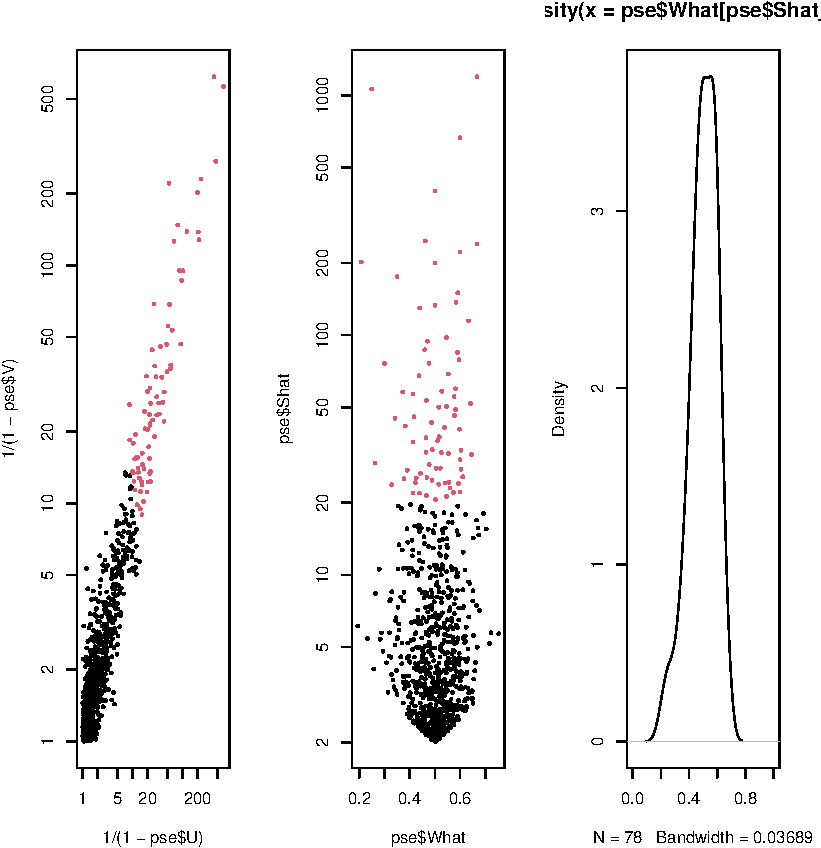
\includegraphics[width=0.7\textwidth,height=\textheight]{mev_files/figure-pdf/unnamed-chunk-1-1.pdf}

}

\caption{Figure: Extremal dependence.}

\end{figure}%

\section{Clustering Methods in
Extremes}\label{clustering-methods-in-extremes}

\begin{itemize}
\item
  Handbook on Statistics of Extremes 책 발간 예정
\item
  Vector quantization
\end{itemize}

\subsection{K-means clustering}\label{k-means-clustering}

\begin{itemize}
\item
  Given obs \(\pmb{x}_1, \ldots, \pmb{x}_n\), find \(K\) cluster
  centroids \(\pmb{c}_1, \ldots, \pmb{c}_K\) s.t. the avg
  data-point-to-centroid dist is minimized: \[
  (\pmb{c}_1, \ldots, \pmb{c}_K) := \arg\min_{\pmb{c}_1, \ldots, \pmb{c}_K} \sum_{k=1}^K 
  \]
\item
  Estimate the centroids \(\pmb{c}_k\) and the cluster membership of
  each \(\pmb{x}_i\) in turns.

  \begin{itemize}
  \tightlist
  \item
    Given \(\hat{\pmb{c}}_1, \ldots, \hat{\pmb{c}}_K\), assign
    \(\pmb{x}_i\) to the cluster \(k\) with the closest centroid
    \(\hat{\pmb{c}}_k\). \[
    i \in C_k \Longleftrightarrow d(\pmb{x}_i, c_k) = \min_{k'}d(\pmb{x}_i, \pmb{c}_{k'})
    \]
  \item
    Given all \(\pmb{x}_i\)'s in cluster \(k\), update each
    \(\hat{\pmb{c}}_k\)
  \end{itemize}
\end{itemize}

\textbf{Q}. Choice of \(d(\cdot, \cdot)\): + Euclidean
\(d(\pmb{x}, \pmb{y}) = (\pmb{x}- \pmb{y})^T(\pmb{x}- \pmb{y})\) + Then
the centroids can be calculated as \[
  \hat{\pmb{c}}_k = \arg\min_{\pmb{c}} \sum_{i\in C_k}(\pmb{x}_i - \pmb{c})^T(\pmb{x}_i - \pmb{c}) = \frac{1}{|C_k|} \sum_{i\in C_k}
  \]

\textbf{Q}. Choice of \(K\): + Prespecified + Use a scree plot where the
obj fct \[
  \min_{\pmb{c}_1, \ldots, \pmb{c}_K} \sum_{k=1}^K \sum_{i \in C_k} d(\pmb{x}_i , \pmb{c}_k)
  \]

이러한 \(K\)-mean 같이 Euclidean dist를 쓰는 방법은 extreme value에서
통하기 어려움

\section{Spectral Clustering}\label{spectral-clustering}

\begin{itemize}
\item
  Can detect nonlinear cluster patterns
\item
  Can identify noise clusters
\end{itemize}

\section{Clustering the Angluar
Components}\label{clustering-the-angluar-components}

\begin{itemize}
\item
  \(\pmb{Y}\) be multivariate regularly varying with standardized margin
  (Frechet 등이 해당) Then \[
  \frac{\pmb{Y}}{\|\pmb{Y}\|}_{\| \pmb{Y}\|>t}\stackrel{d}{\rightarrow} \Theta, \quad{} t \rightarrow \infty.
  \]
\item
  Clustering for extremes:

  \begin{itemize}
  \tightlist
  \item
    Obtain angular compts \(\Theta_1, \ldots, \Theta_{k_n}\) from
    \(\pmb{Y}_1, \ldots , \pmb{Y}_n\)
  \item
    Cluster \(\Theta_1, \ldots, \Theta_{k_n}\) instead.
  \end{itemize}
\end{itemize}

여기서 \(\Theta\)는 unit sphere \(\{ \pmb{x} \| \pmb{x} \| = 1\}\)이라는
매우 좋은 space에 놓여 있다. (이때 \(\| \cdot \|\)은 any norm이나 되지만
\(L2\) norm을 쓰기로 한다)

\section{Max-Linear Models}\label{max-linear-models}

\begin{itemize}
\item
  Max-linear random vector: \[
  \pmb{X} = (X_1, \ldots, X_d) = \vee_{i=1, \ldots, K}\pmb{b}_i Z_i
  \]
\item
  Factors \(\pmb{b}_1, \ldots, \pmb{b}_{K} \in [ 0, \infty )^{d}\)
\item
  \(Z_1, \ldots, Z_k\): i.i.d. Frechet
\end{itemize}

Then the angular measure \(\Theta\) consists of point masses at \[
\frac{\pmb{b}_1}{\|\pmb{b}_1\|}, \ldots
\]

\subsection{\texorpdfstring{Spherical
\(K\)-means}{Spherical K-means}}\label{spherical-k-means}

\begin{itemize}
\tightlist
\item
  Apply to \(\Theta_1, \ldots, \Theta_{k_n}\): \(K\)-means clustering
  with choice of distance \[
  d(\pmb{x}, \pmb{y}) = 1- \cos (\pmb{x}, \pmb{y})
  \]
\end{itemize}

On the unit sphere \(\mathbb{S}_{+}^{d-1}\),

\begin{itemize}
\tightlist
\item
  \(d(\pmb{x}, \pmb{y})= 1-\pmb{x}^T\pmb{y}\)
\item
  \(d\) is equiv to the Euclidean dist
\end{itemize}

\subsection{\texorpdfstring{Spherical \(K\)-PCs clustering for
extremes}{Spherical K-PCs clustering for extremes}}\label{spherical-k-pcs-clustering-for-extremes}

\begin{itemize}
\item
  앞선 방법과 달리 \(d(\pmb{x}, \pmb{y}) = 1-(\pmb{x}^T\pmb{y})^2\)을
  쓰는 것이 차이점(제곱이 들어감)
\item
  https://academic.oup.com/biomet/article-abstract/110/1/135/6551983?redirectedFrom=PDF
\item
  \(\arg\max_{\|\pmb{c}\|_2=1} \pmb{c}^T\Sigma_k \pmb{c}\) 형태가 나옴
\item
  For any spectral measure that can be decomposed into two sub-faces
  \(l_1\) and \(l_2\), we would like the optimal centroids to satisfy \[
  \pmb{c}_1 \in \mathbb{F}_{l_1}, \quad{} \pmb{c}_2 \in \mathbb{F}_{l_2}
  \]
\item
  This holds for spheical \(K\)-means iff \[
  \|l_1 | - | l_2 \| \leq 1
  \]
\item
  This holds for spherical \(K\)-PCs always.
\item
  If angular components \(\pmb{x}\) and \(\pmb{y}\) belongs to different
  sub-faces, then \(\pmb{x}^T\pmb{y}\) close to \(0\).
\end{itemize}

\subsection{Spectral clustering for
extremes}\label{spectral-clustering-for-extremes}

\begin{itemize}
\tightlist
\item
  Linear factor model with noise: \[
  \pmb{X} = (X_1, \ldots, X_d) = \sum_{i=1}^K
  \]
\end{itemize}

\part{Intro}

\chapter{Summary}\label{summary}

In summary, this book has no content whatsoever.

\begin{Shaded}
\begin{Highlighting}[]
\DecValTok{1} \SpecialCharTok{+} \DecValTok{1}
\end{Highlighting}
\end{Shaded}

\begin{verbatim}
[1] 2
\end{verbatim}

\chapter*{References}\label{references-1}
\addcontentsline{toc}{chapter}{References}

\markboth{References}{References}

\phantomsection\label{refs}
\begin{CSLReferences}{1}{0}
\bibitem[\citeproctext]{ref-Durrett2019}
Durrett, Rick. 2019. \emph{Probability: Theory and Examples}. 5th ed.
Cambridge University Press.
\url{https://www.ebook.de/de/product/34699864/rick_duke_university_north_carolina_durrett_probability.html}.

\bibitem[\citeproctext]{ref-Gut2014}
Gut, Allan. 2014. \emph{Probability: A Graduate Course}. 2nd ed.
Springer New York.

\bibitem[\citeproctext]{ref-Polansky2011}
Polansky, Alan M. 2011. \emph{Introduction to Statistical Limit Theory}.
CRC Press.

\end{CSLReferences}



\end{document}
